\begin{appendices}

More info can be found here: https://github.com/daniel-leonard-robinson/thesis

%\chapter{Bill of Materials}
%\label{app:bom}
%
%\begin{itemize}
%	\item F450 frame
%	\item Motors
%	\item 
%\end{itemize}

\chapter{Moisture sensor}

A cheap moisture sensor from China was investigated as in Figure \ref{fig:moisture_sensor}. It might be useful if it can be used for ground-truthing.

\begin{figure}[H]
\centering
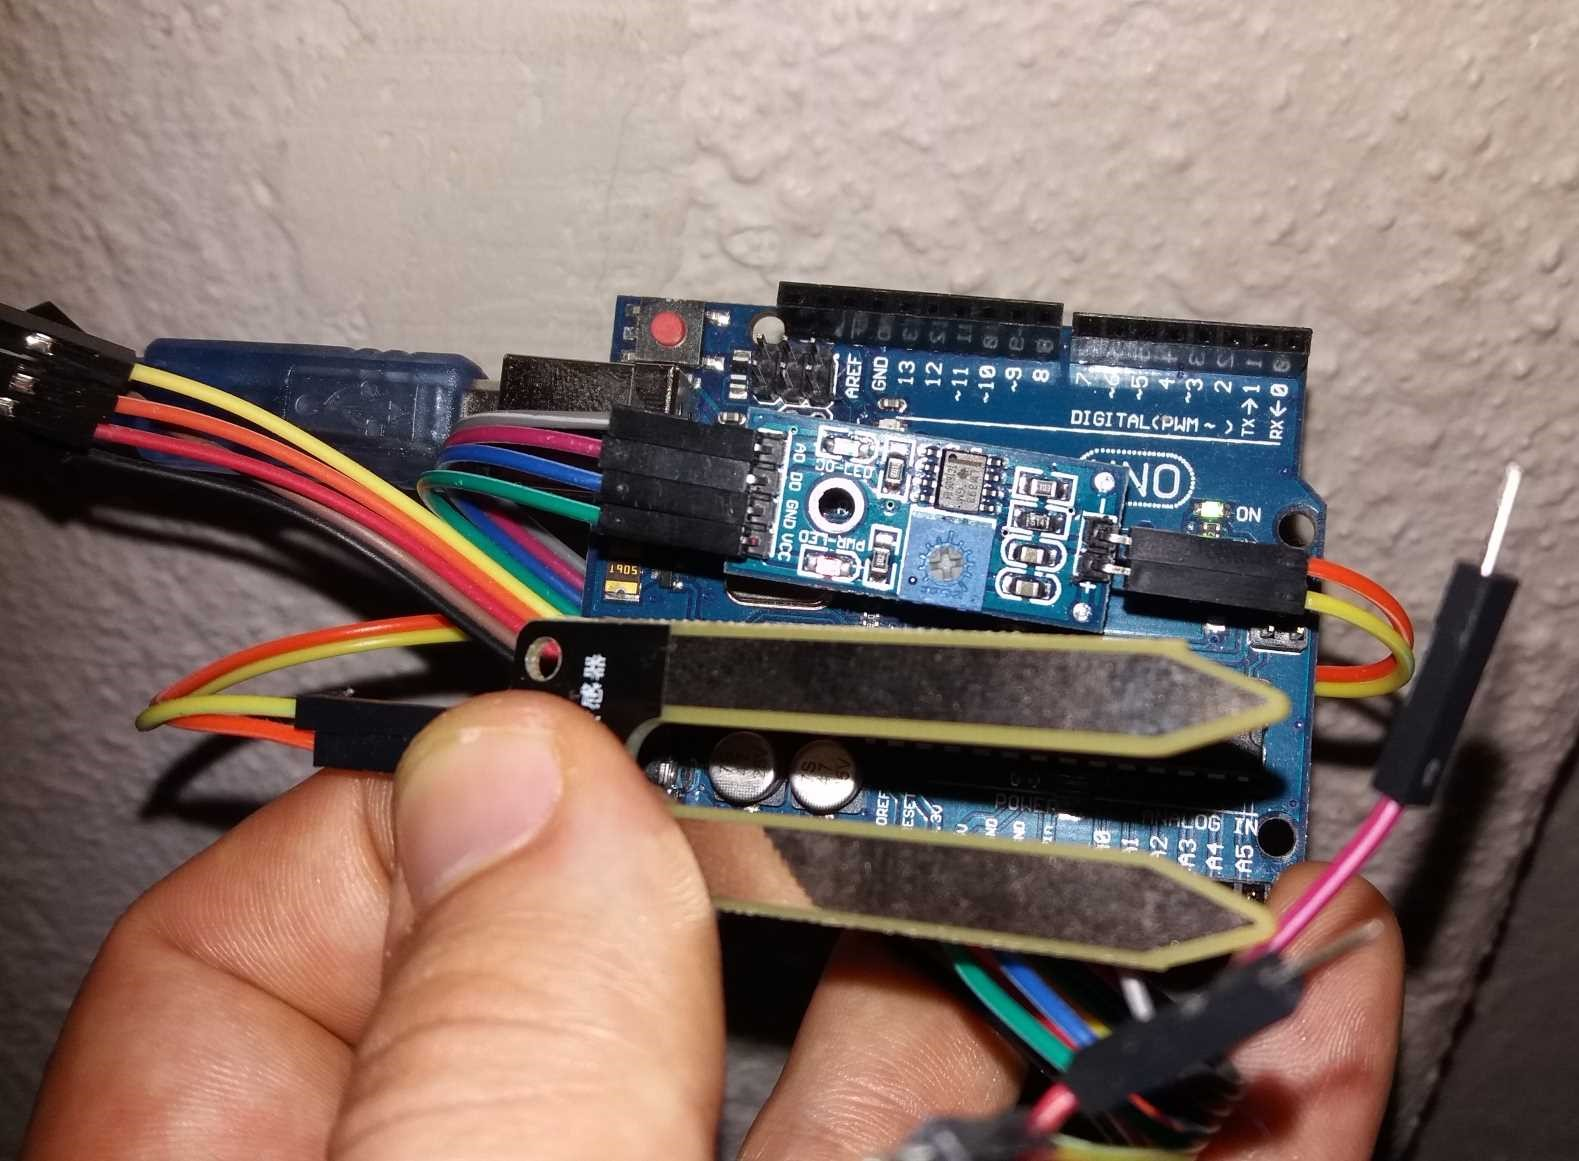
\includegraphics[scale=0.17]{images/moisture_sensor.jpg}
\caption{Moisture sensor}
\label{fig:moisture_sensor}
\end{figure}

The sensor measures the resistivity of the soil, and values range from about 5V for an open circuit, and about 1V for different types of water (salty, brackish etc). A typical soil value would be about 1.5V for wet soil, and 4V for dry soil. Unfortunately, there was too much variance for the same type of soil, and it was determined that more accurate equipment is needed. It is also more expensive, but worth investigating.

\chapter{Spectrum analyzer}

A spectrum analyzer kit was built to investigate what can be found from diffraction and perhaps identifying spectral characteristics of cameras.

\begin{figure}[H]
\centering
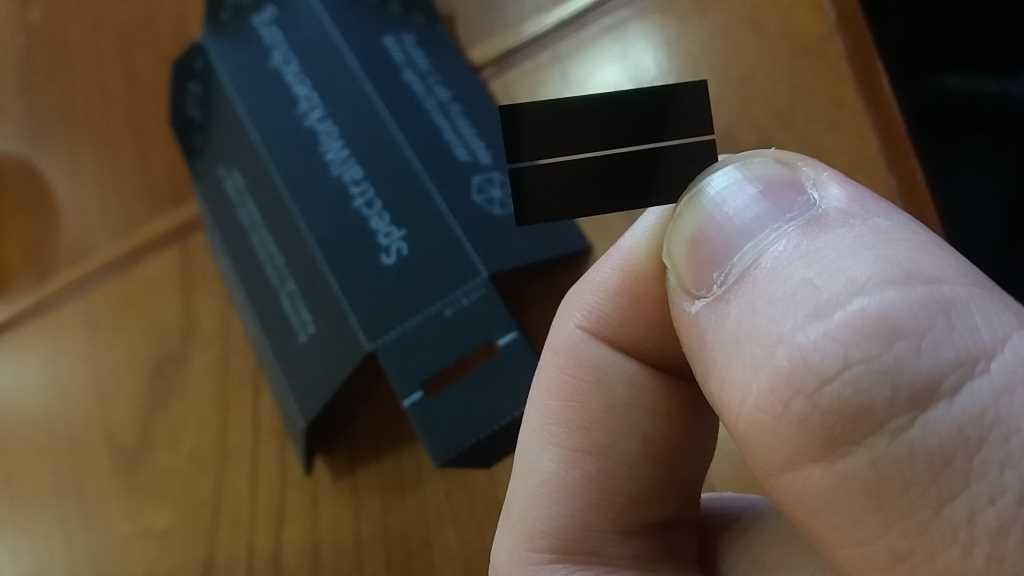
\includegraphics[scale=0.4]{images/collimeter.jpg}
\caption{Acetate collimeter}
\label{fig:coll}
\end{figure}

\begin{figure}[H]
\centering
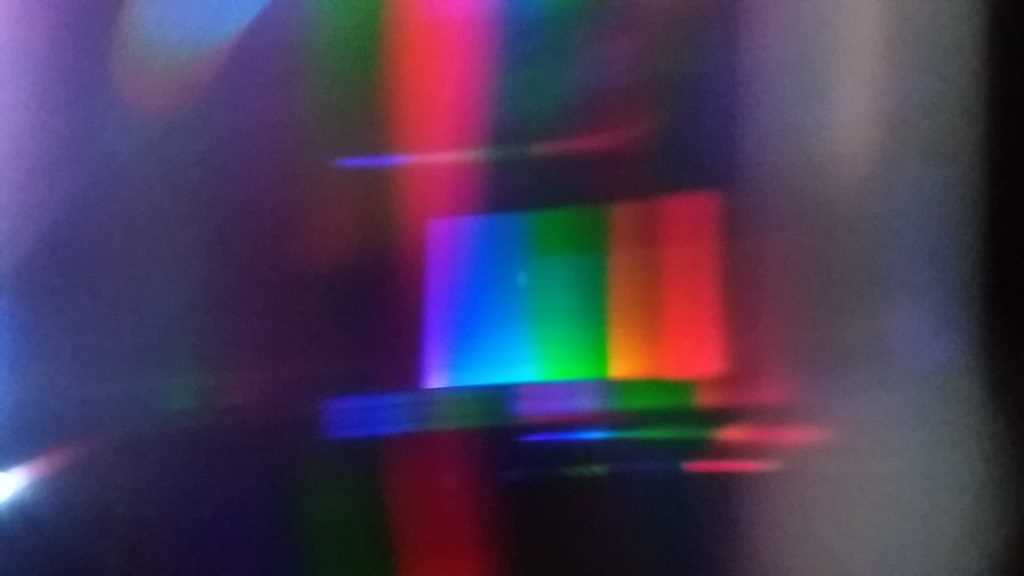
\includegraphics[scale=0.4]{images/spectrum.jpg}
\caption{Diffraction from light source}
\label{fig:diffraction}
\end{figure}

Unfortunately it proved too flimsy, and that laboratory equipment would be better suited.


\chapter{Filter comparison}
\label{app:filter_comparison}

See filters in Section \ref{sec:filters} for an in-depth discussion.

\begin{figure}[H]
\centering
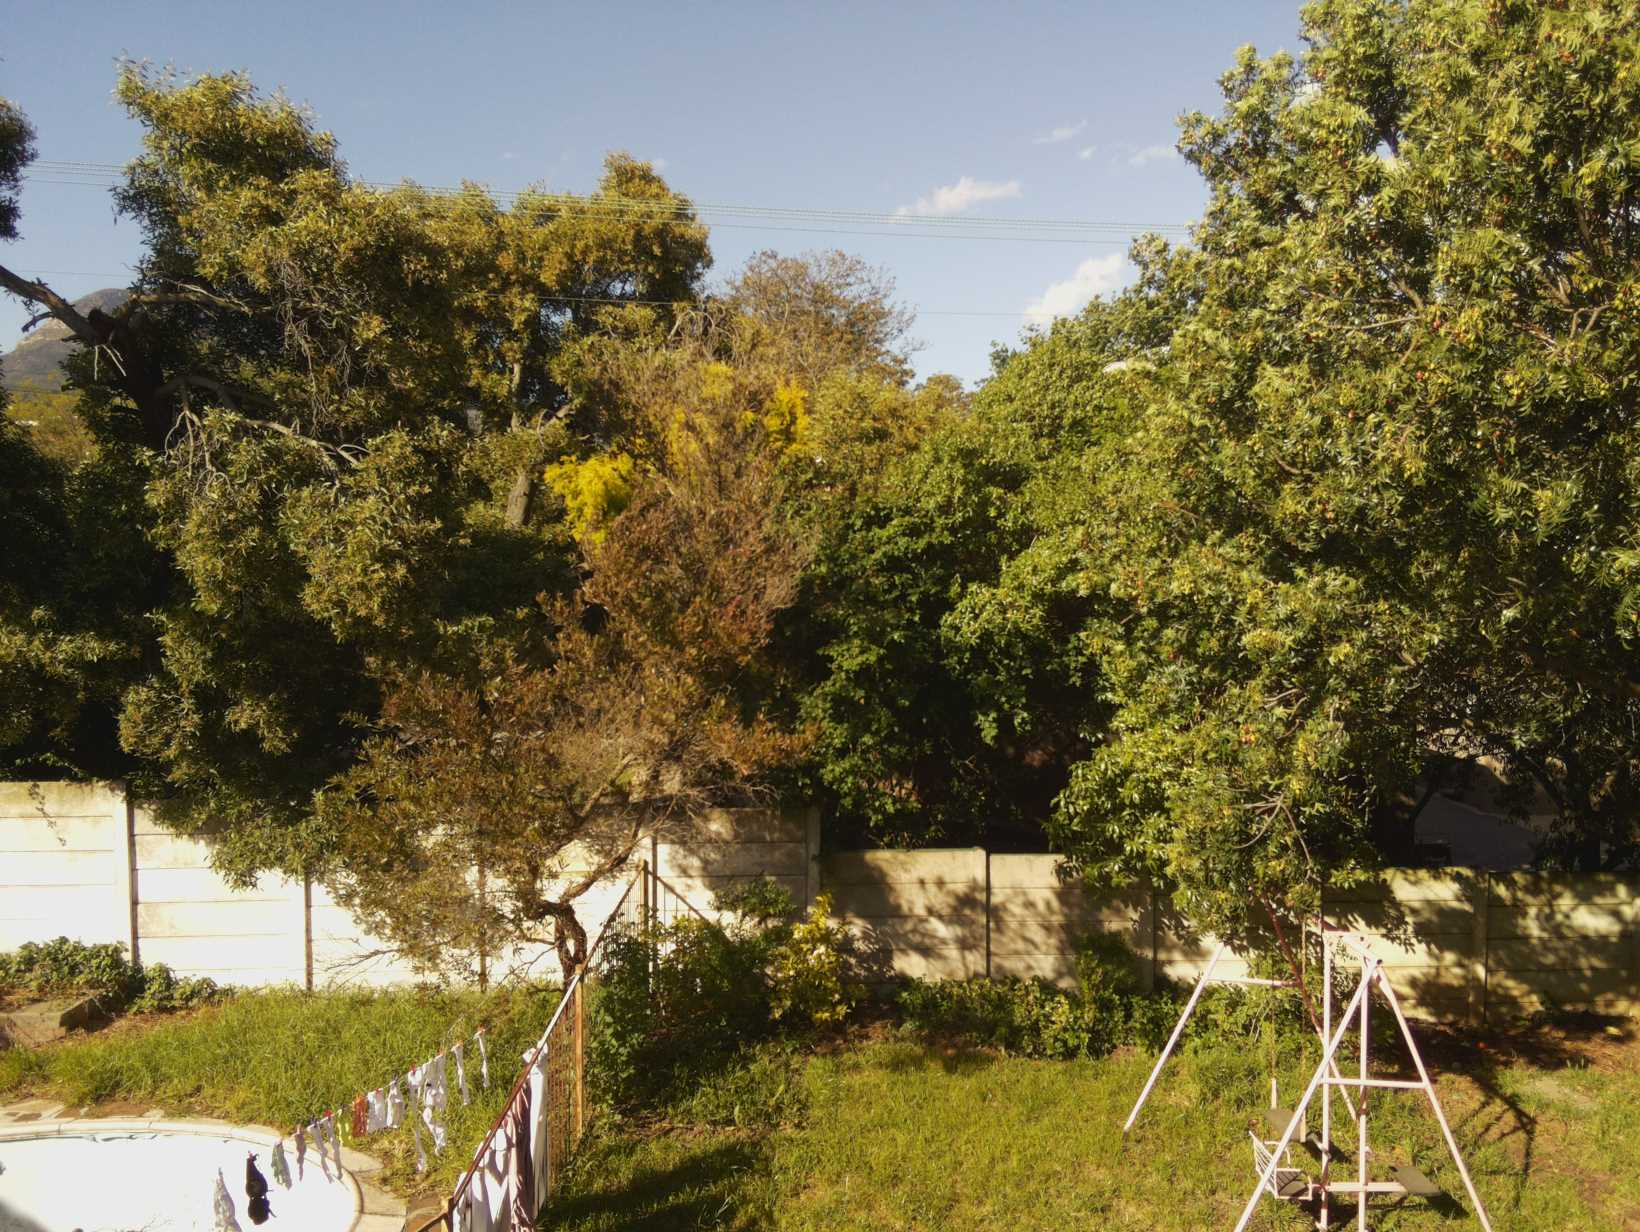
\includegraphics[scale=0.2]{filter/rgb.jpg}
\caption{RGB image overlooking vegetation outside window}
\label{fig:f_rgb}
\end{figure}

\begin{figure}[H]
\begin{subfigure}{0.5\textwidth}
\centering
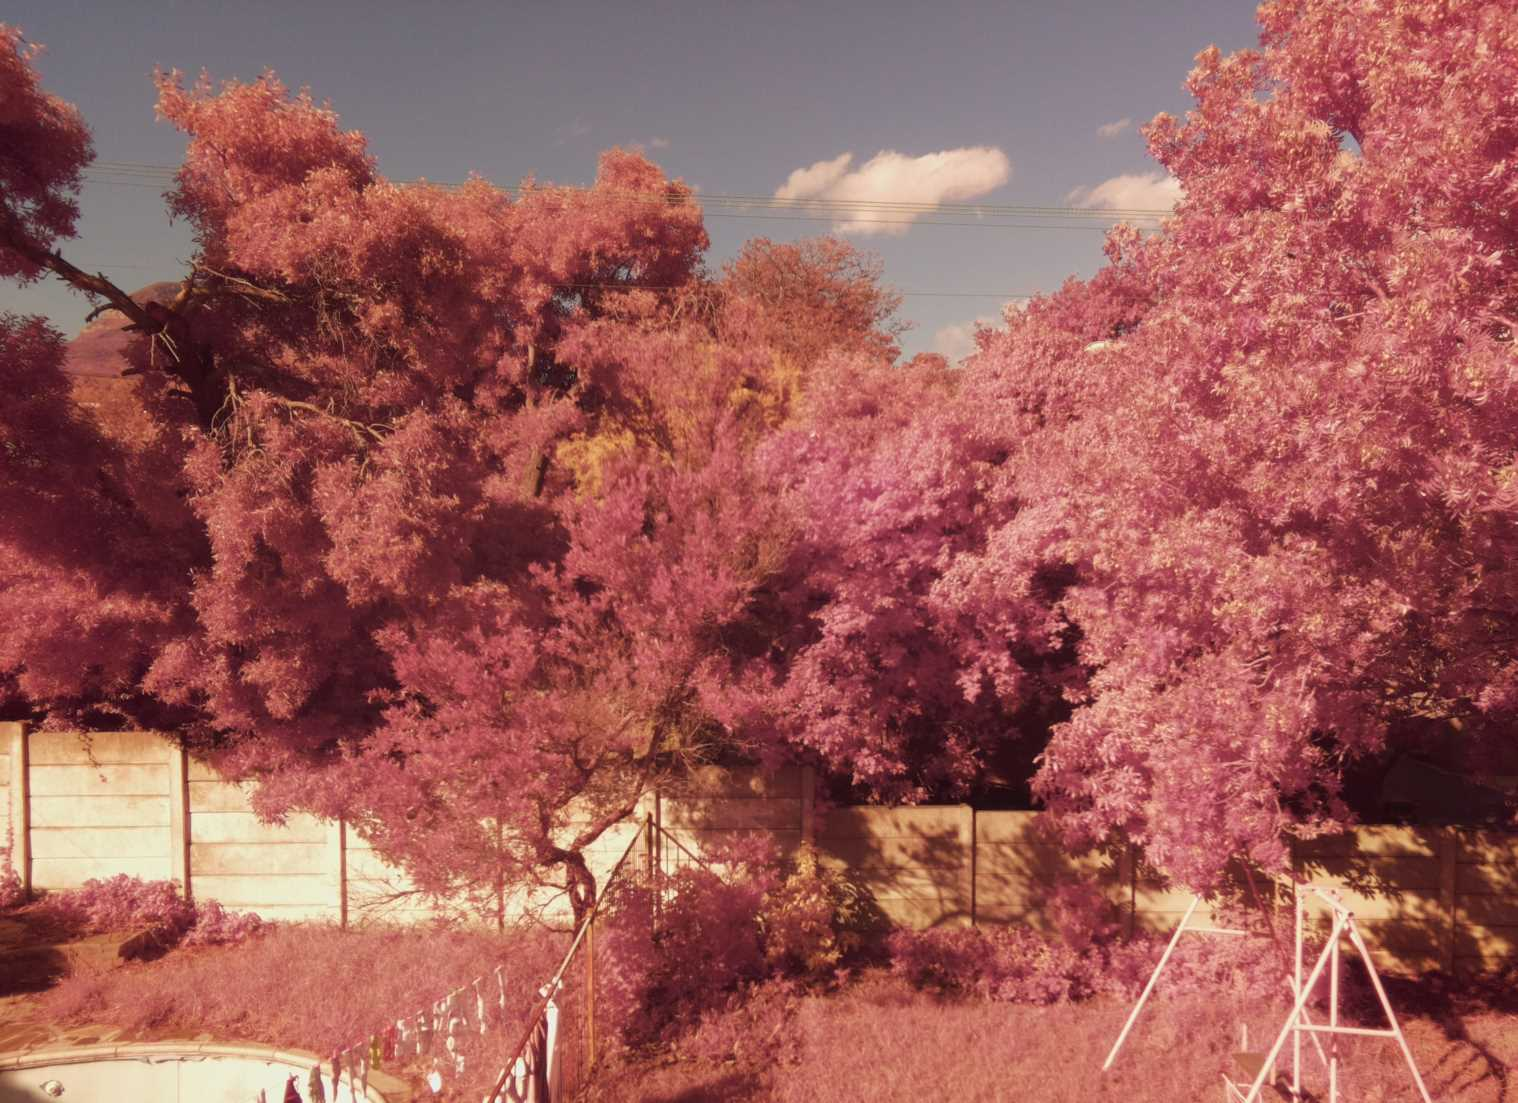
\includegraphics[scale=0.2]{filter/noir.jpg}
\caption{No filter image}
\end{subfigure}
\begin{subfigure}{0.5\textwidth}
\centering
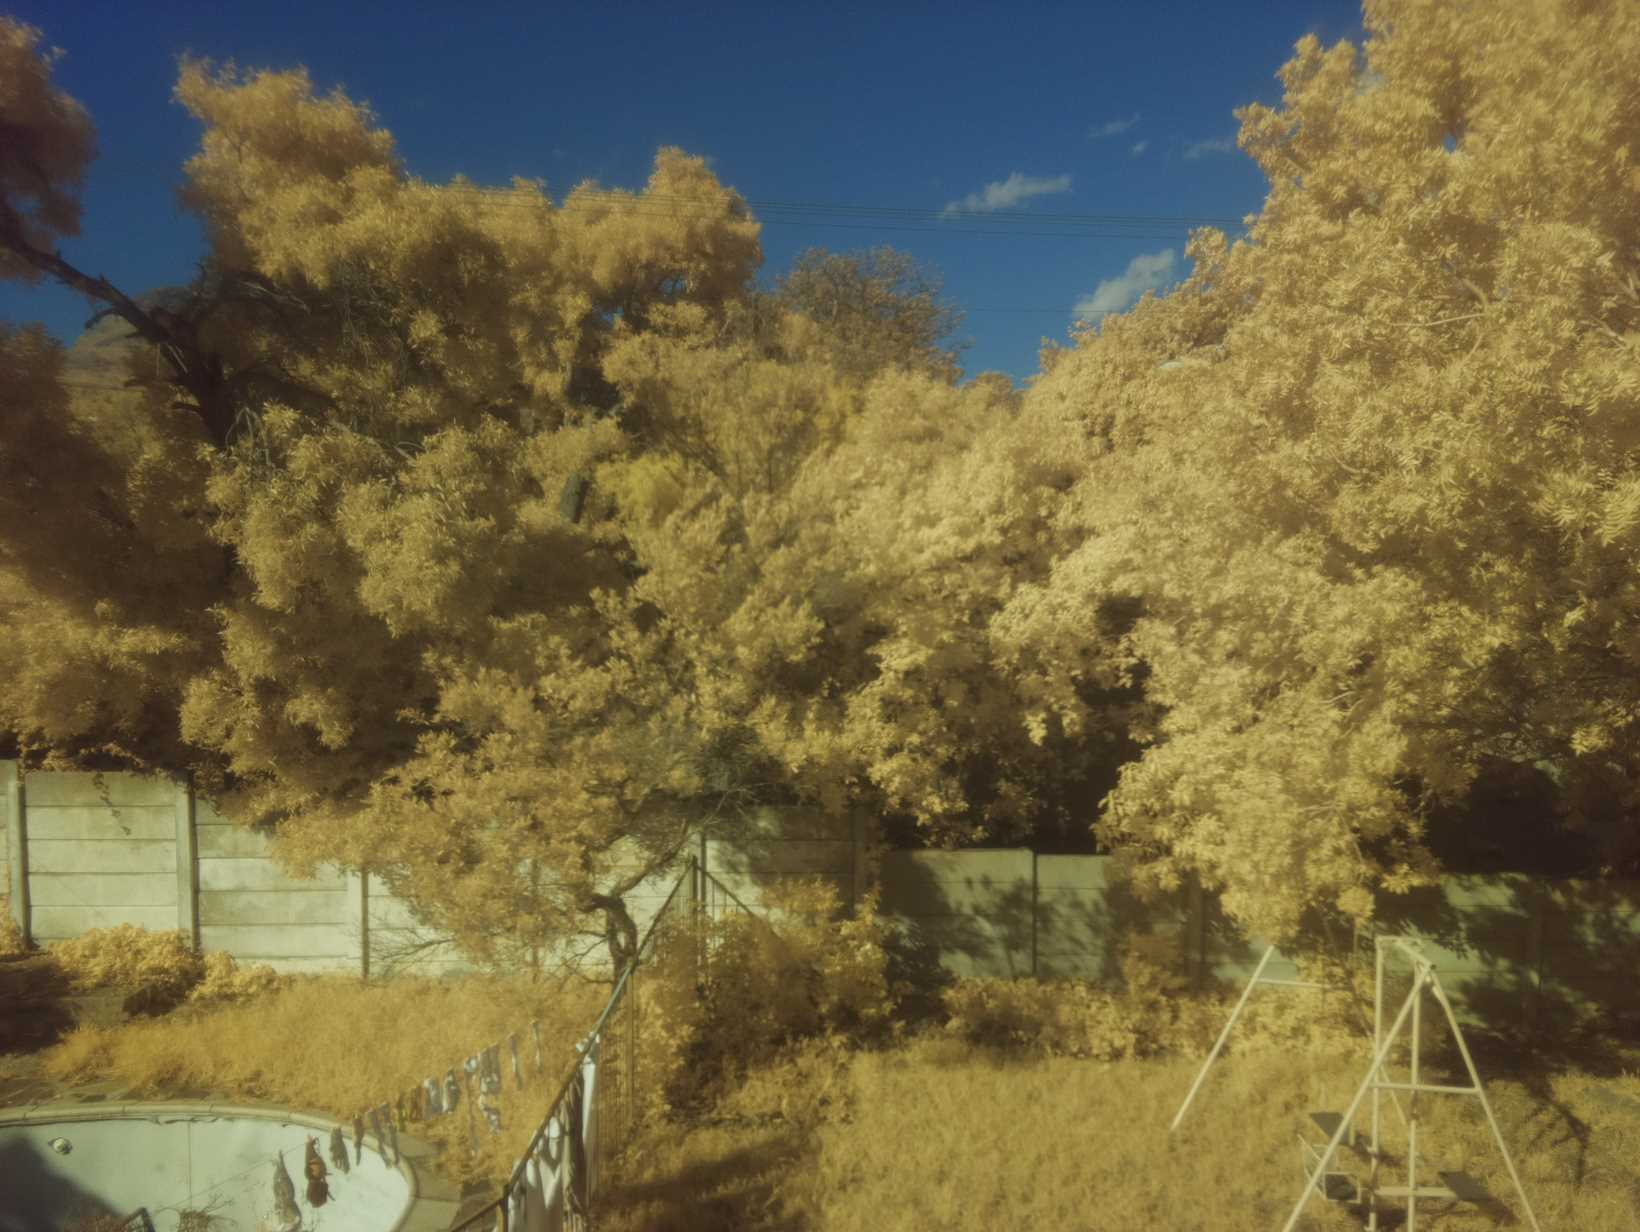
\includegraphics[scale=0.17]{filter/blue_ir.jpg}
\caption{Blue filter image}
\end{subfigure}
\begin{subfigure}{0.5\textwidth}
\centering
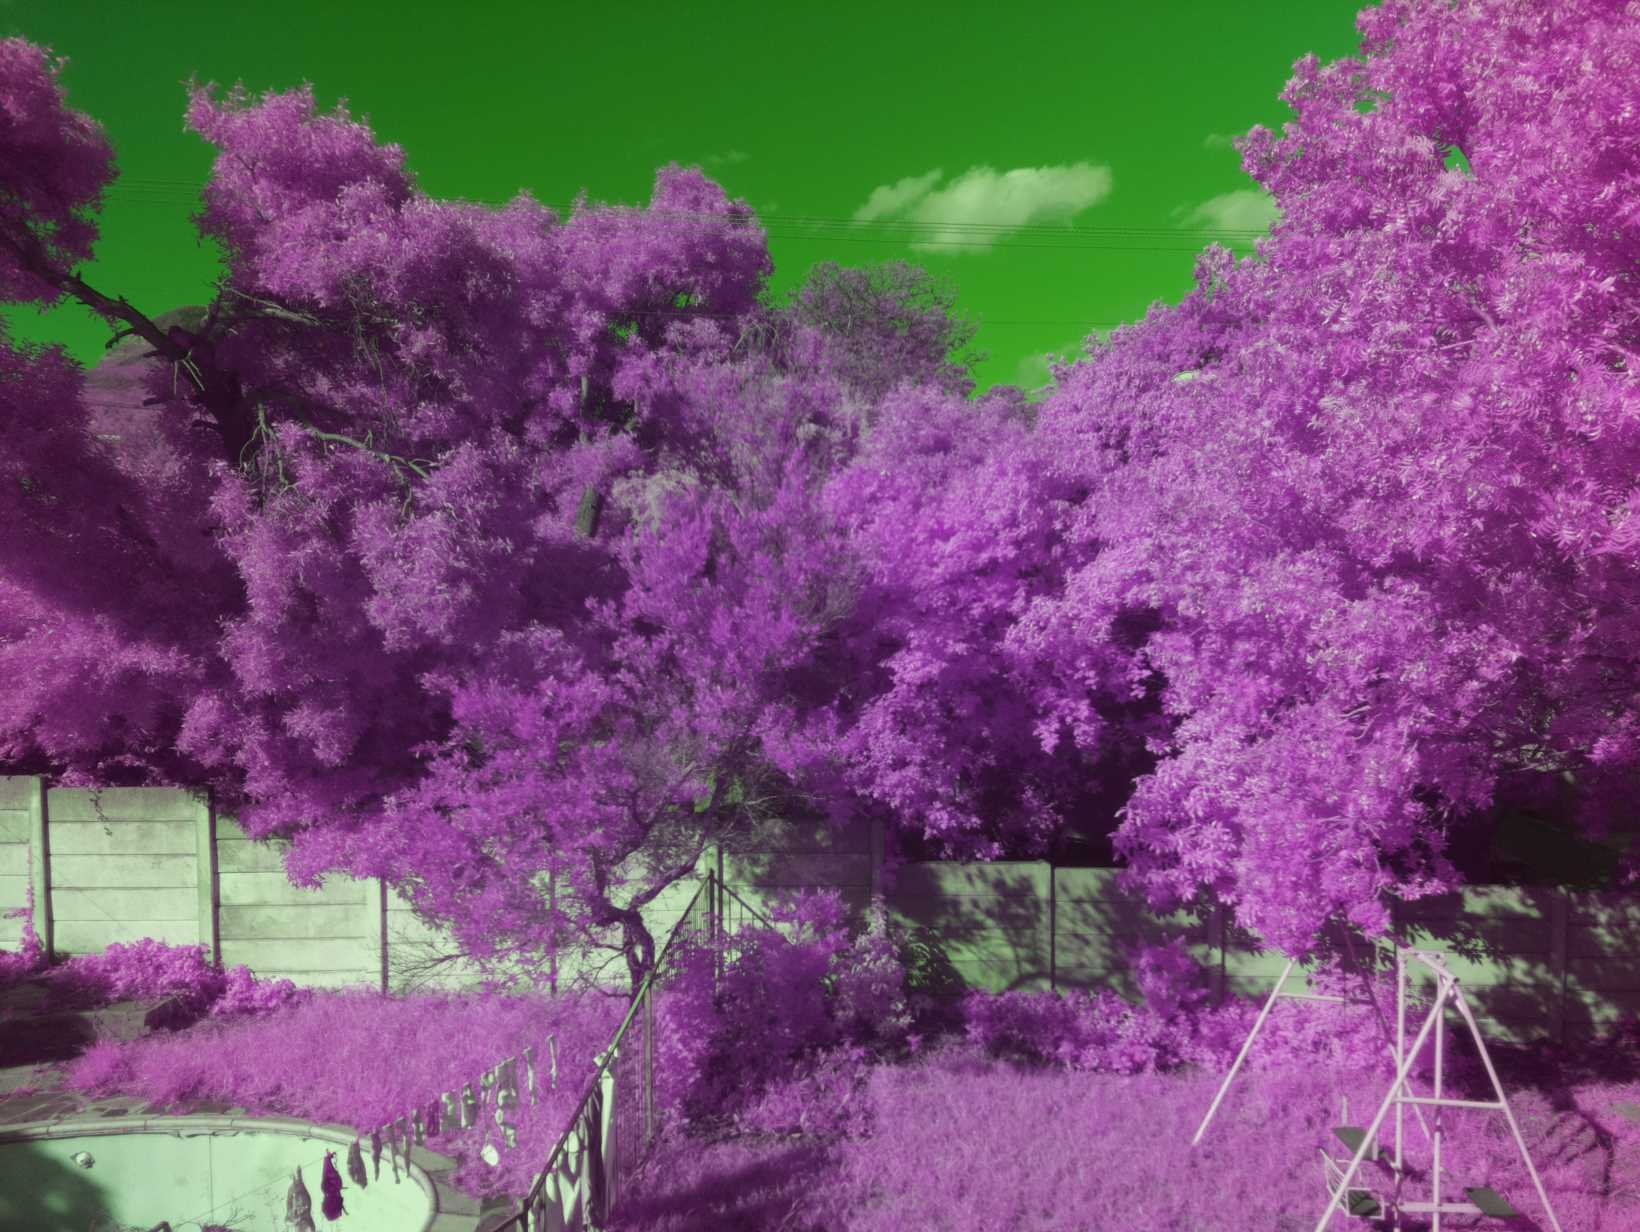
\includegraphics[scale=0.17]{filter/green_ir.jpg}
\caption{Green filter image}
\end{subfigure}
\begin{subfigure}{0.5\textwidth}
\centering
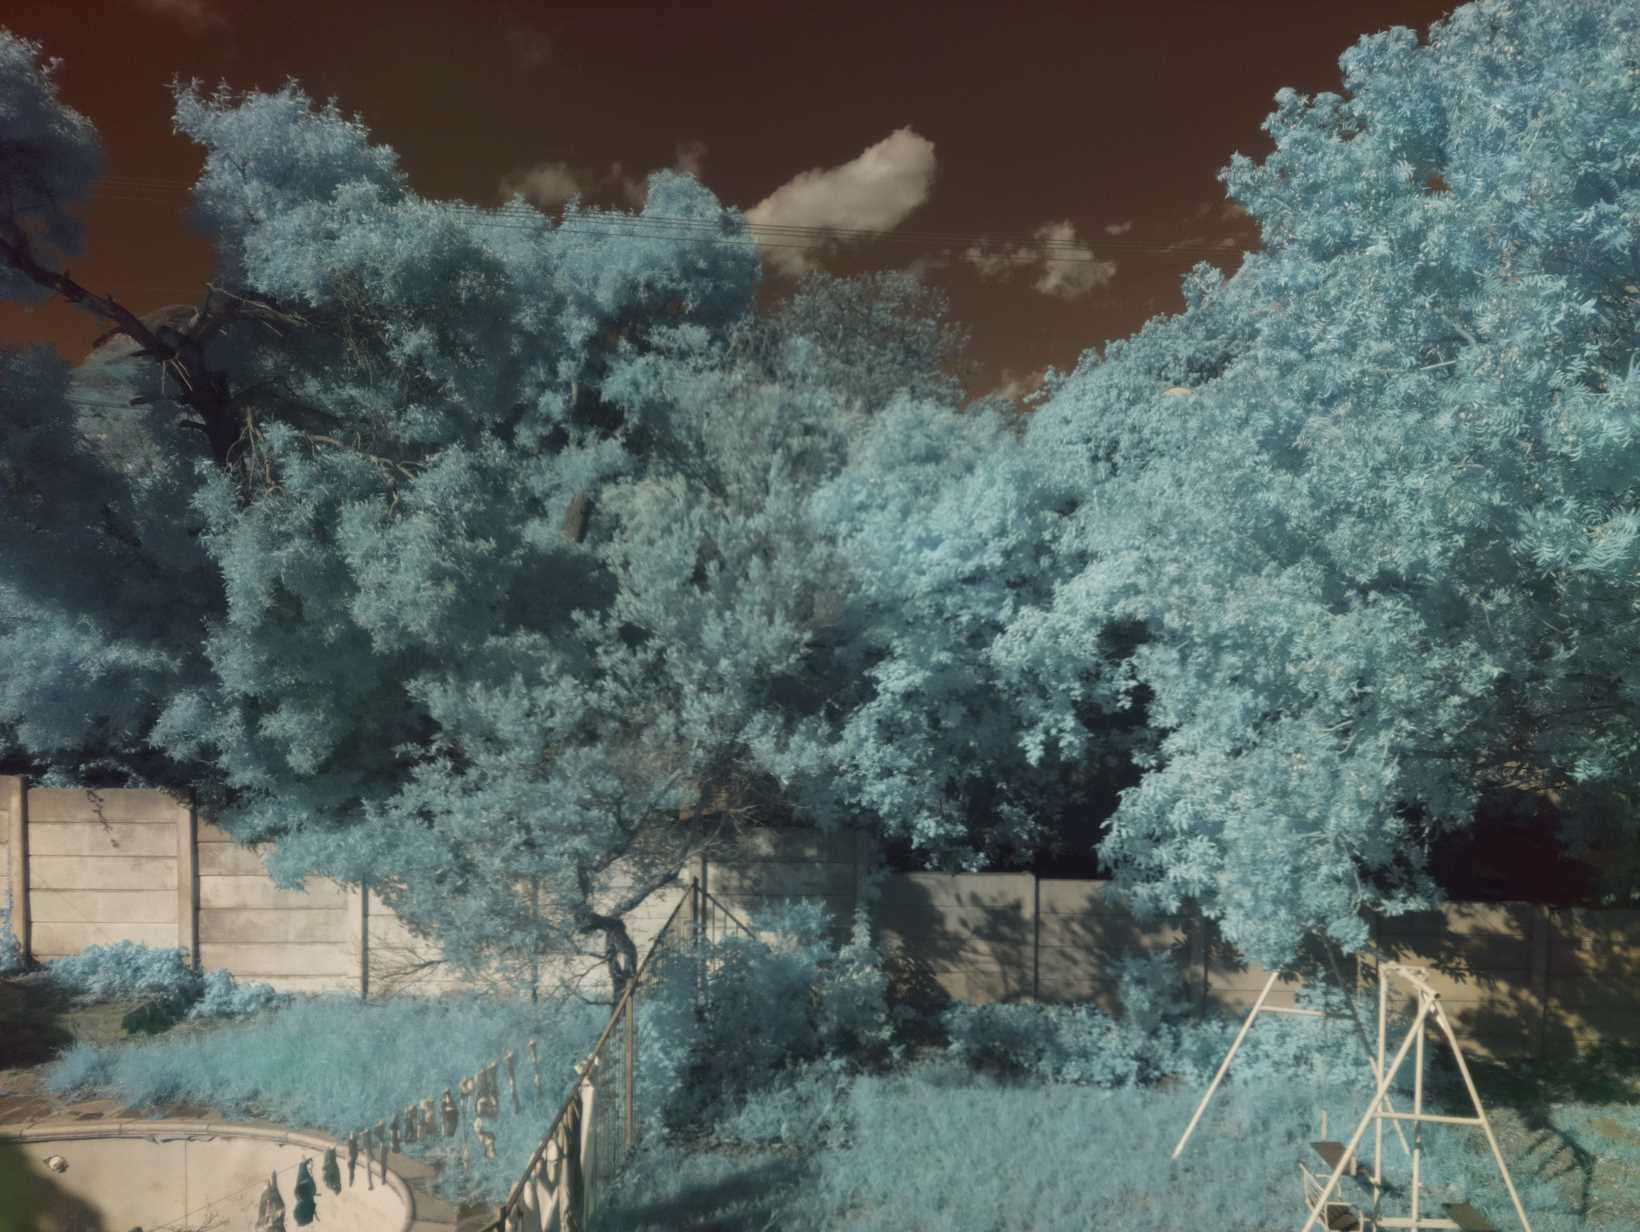
\includegraphics[scale=0.17]{filter/red_ir.jpg}
\caption{Red filter image}
\end{subfigure}
\caption{Filter images}
\label{fig:filters}
\end{figure}

In Figure \ref{fig:filters_ndvis}, the $=$ sign denotes which channel the $NIR$ and $VIS$ of Equation \ref{eq:ndvi} uses.

\begin{figure}[H]
\begin{subfigure}{0.5\textwidth}
\centering
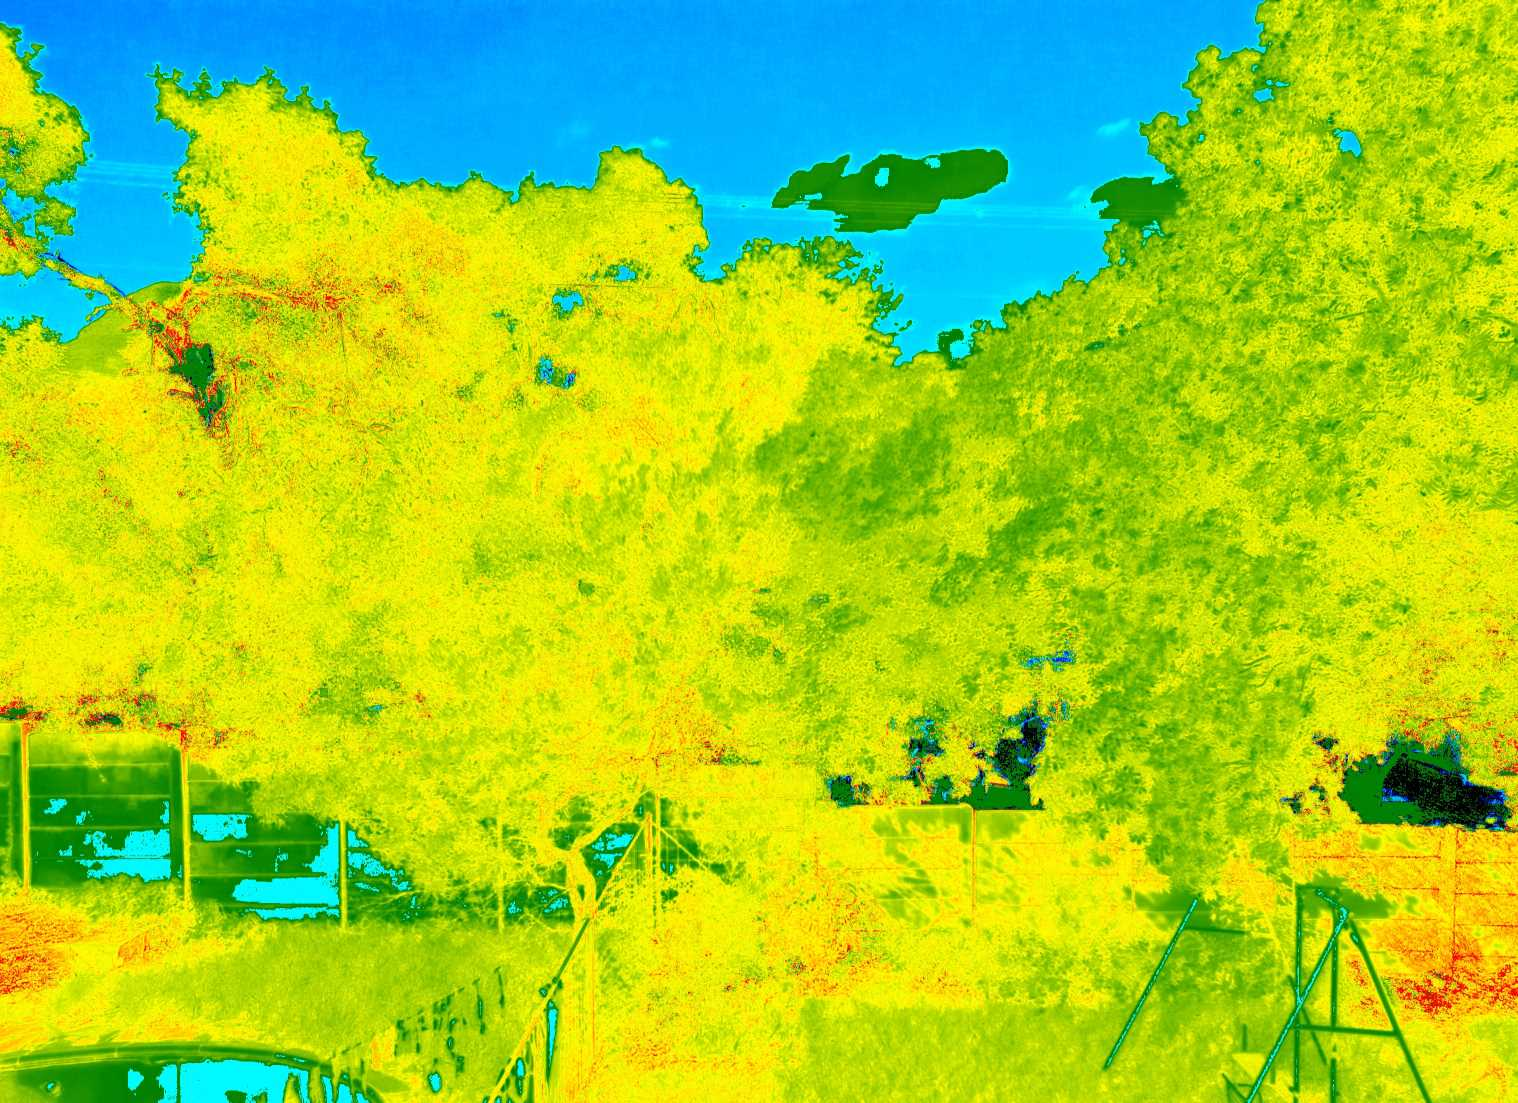
\includegraphics[scale=0.17]{filter/noir_Color_Index.jpg}
\caption{No filter NDVI (NIR=red, VIS=blue)}
\end{subfigure}
\begin{subfigure}{0.5\textwidth}
\centering
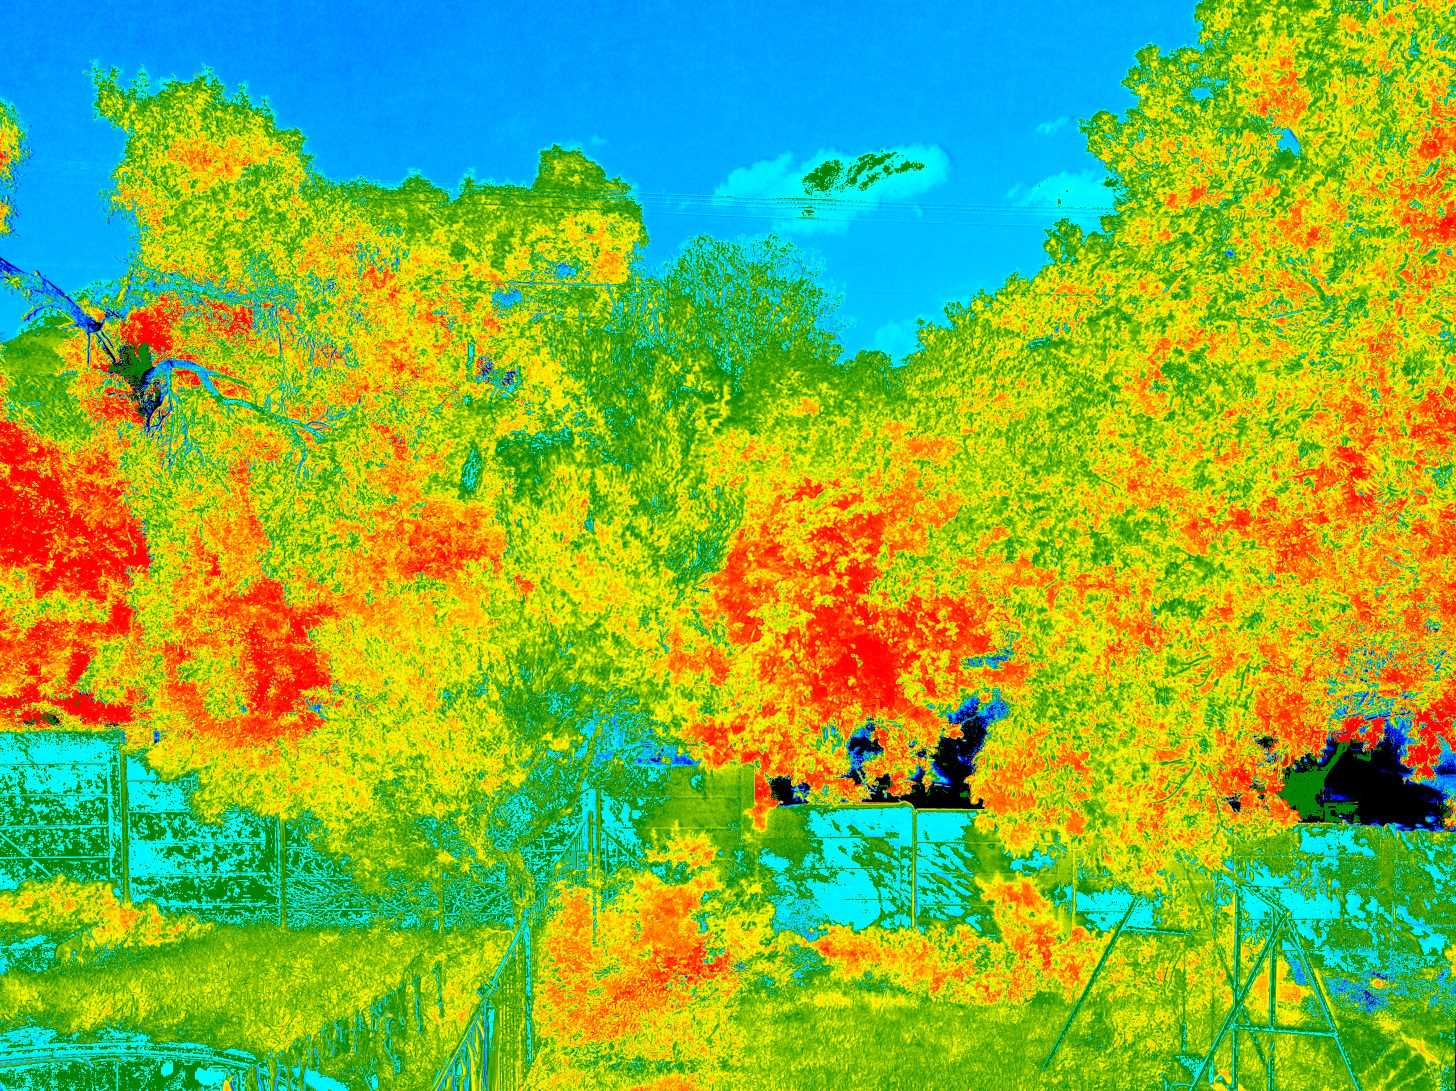
\includegraphics[scale=0.17]{filter/noir_d_ndvi.jpg}
\caption{No filter NDVI (NIR=red, VIS=red)}
\end{subfigure}
\begin{subfigure}{0.5\textwidth}
\centering
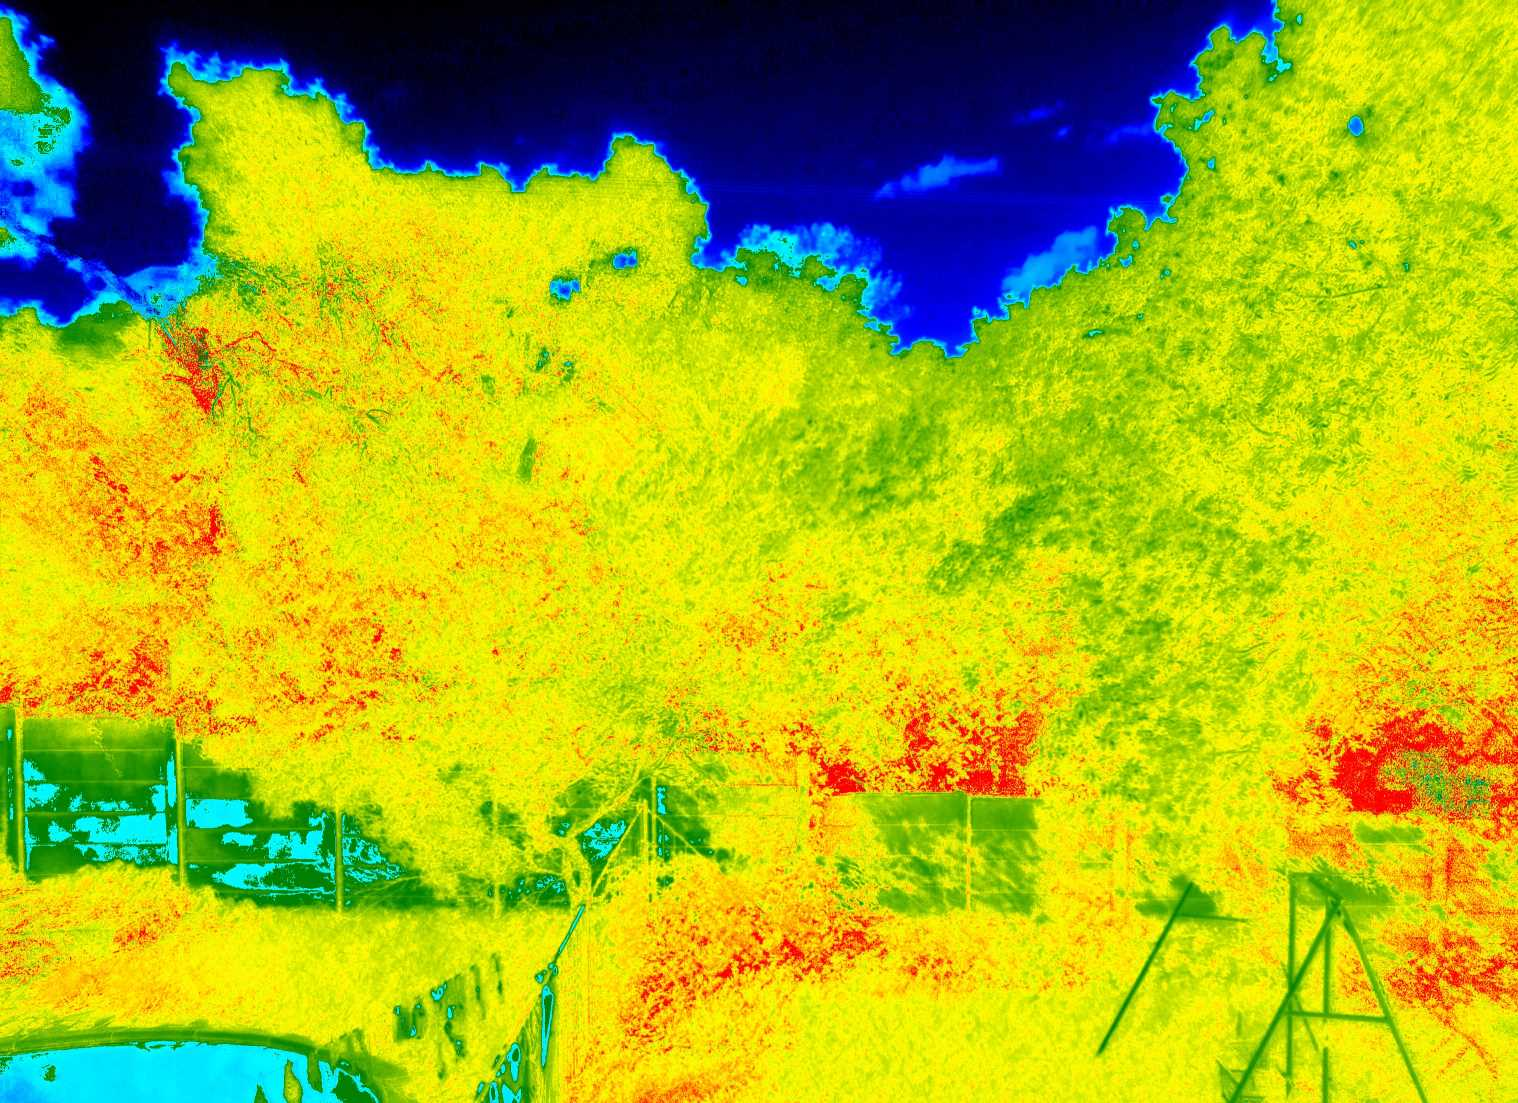
\includegraphics[scale=0.17]{filter/blue_Color_Index.jpg}
\caption{Blue filter NDVI (NIR=red, VIS=blue)}
\end{subfigure}
\begin{subfigure}{0.5\textwidth}
\centering
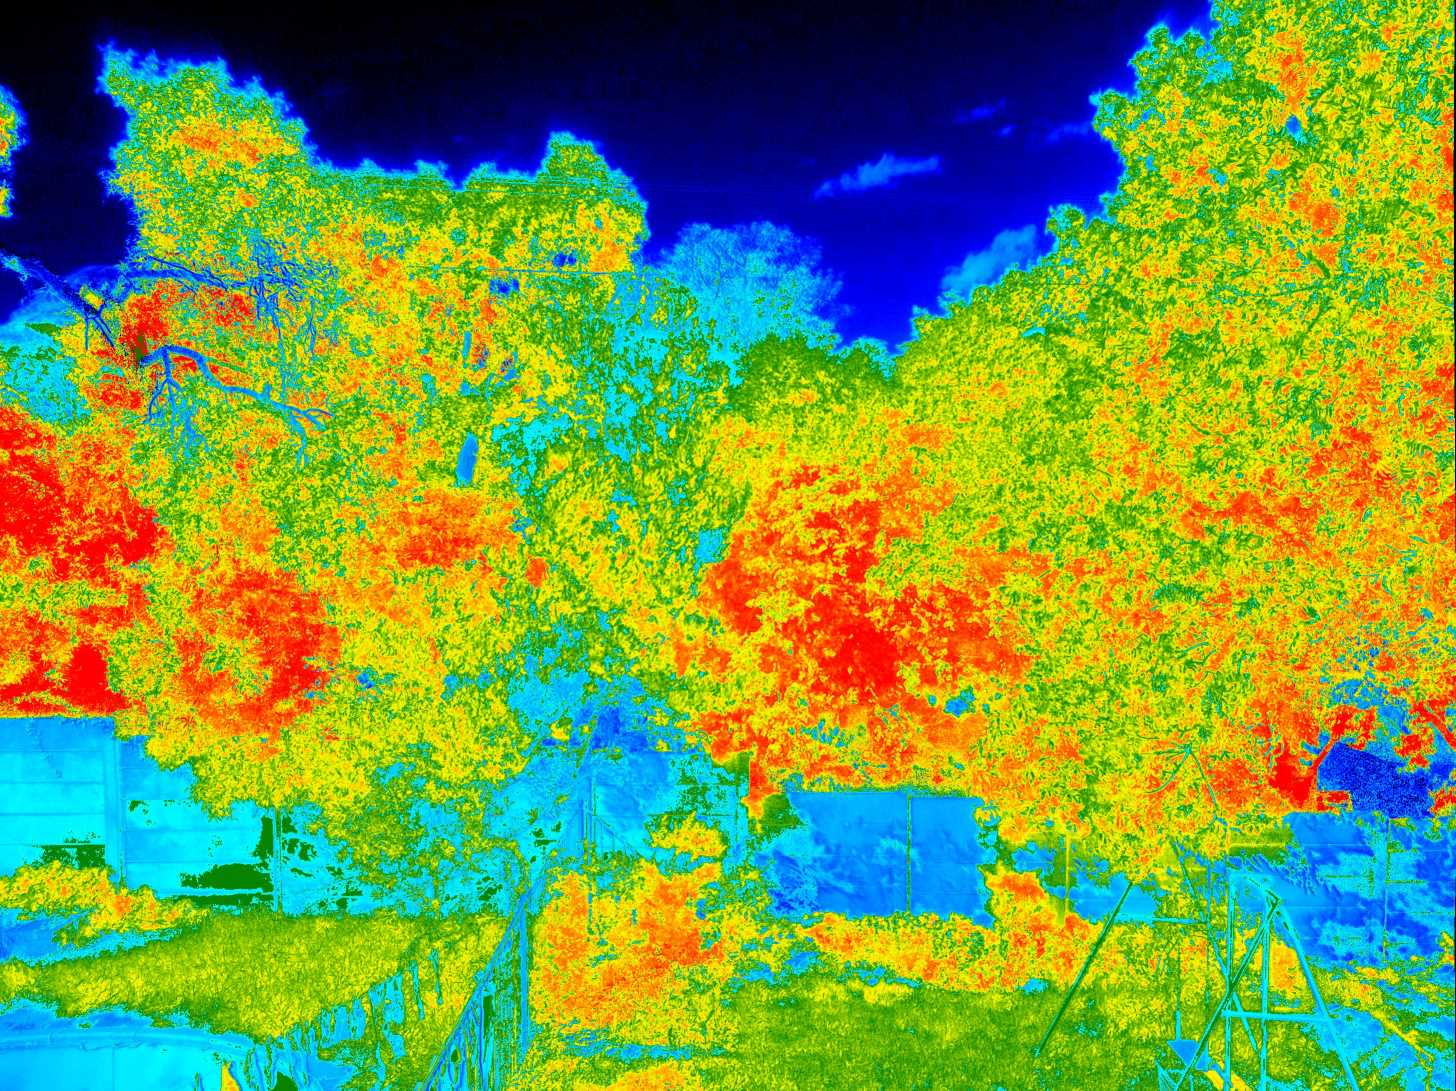
\includegraphics[scale=0.17]{filter/blue_d_ndvi.jpg}
\caption{Blue filter NDVI (NIR=red, VIS=red)}
\end{subfigure}
\begin{subfigure}{0.5\textwidth}
\centering
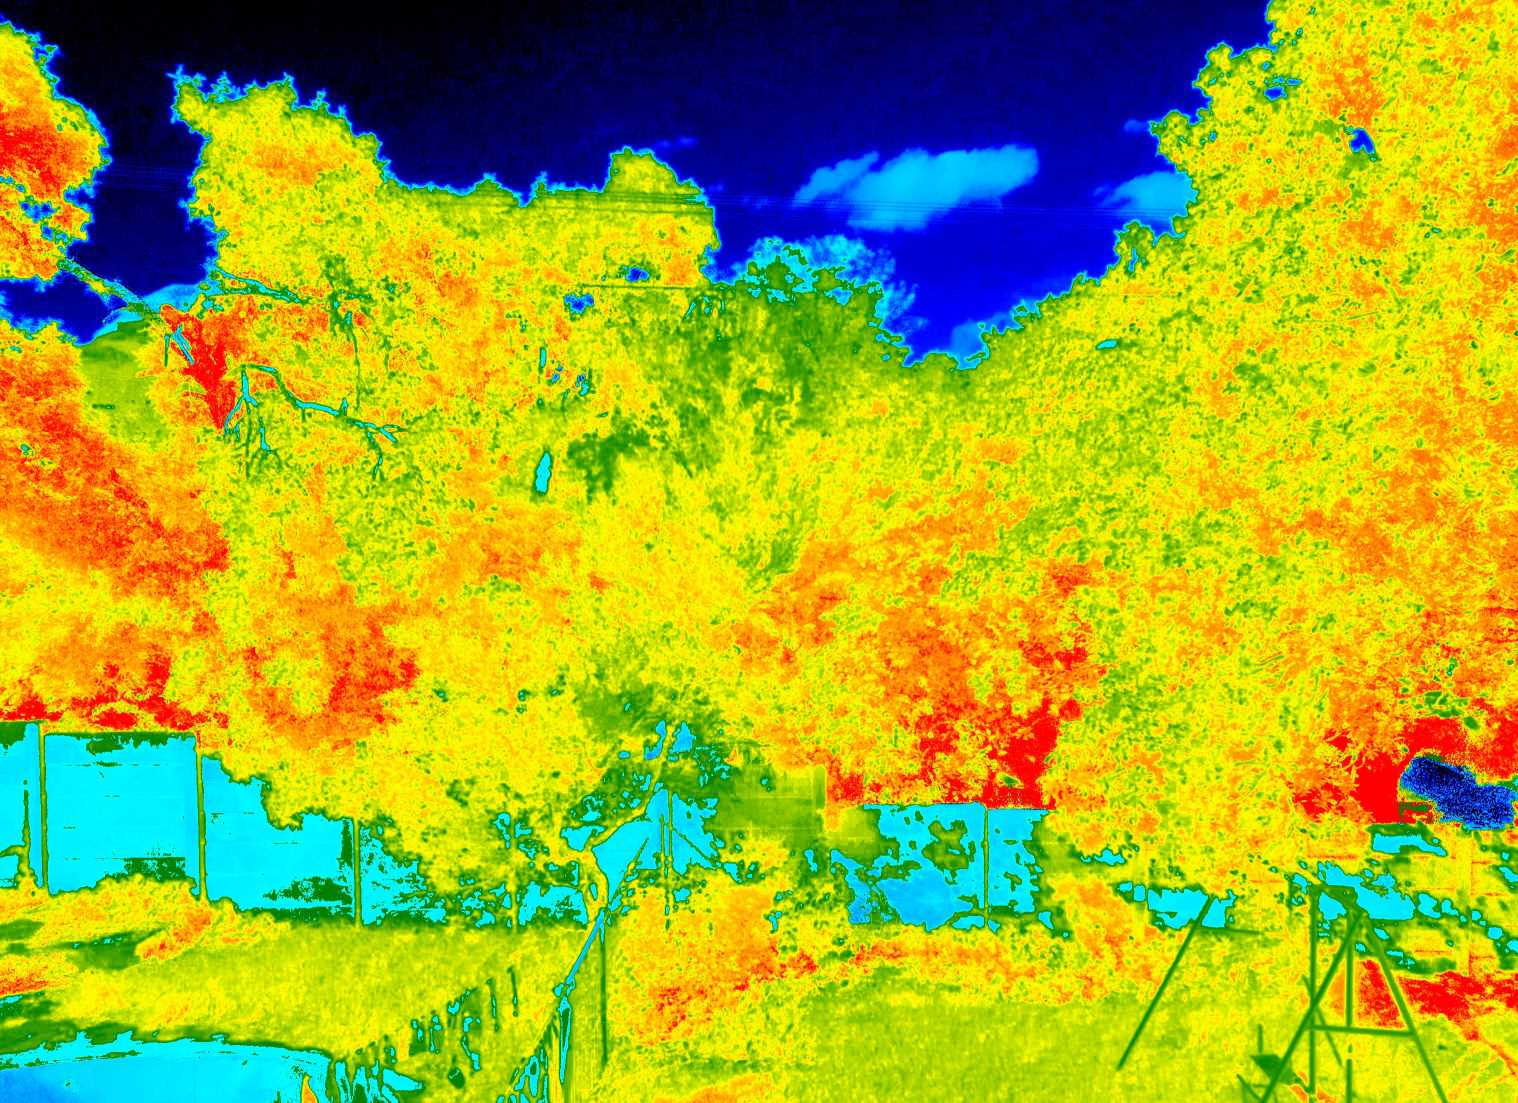
\includegraphics[scale=0.17]{filter/green_Color_Index.jpg}
\caption{Green filter NDVI (NIR=red, VIS=green)}
\end{subfigure}
\begin{subfigure}{0.5\textwidth}
\centering
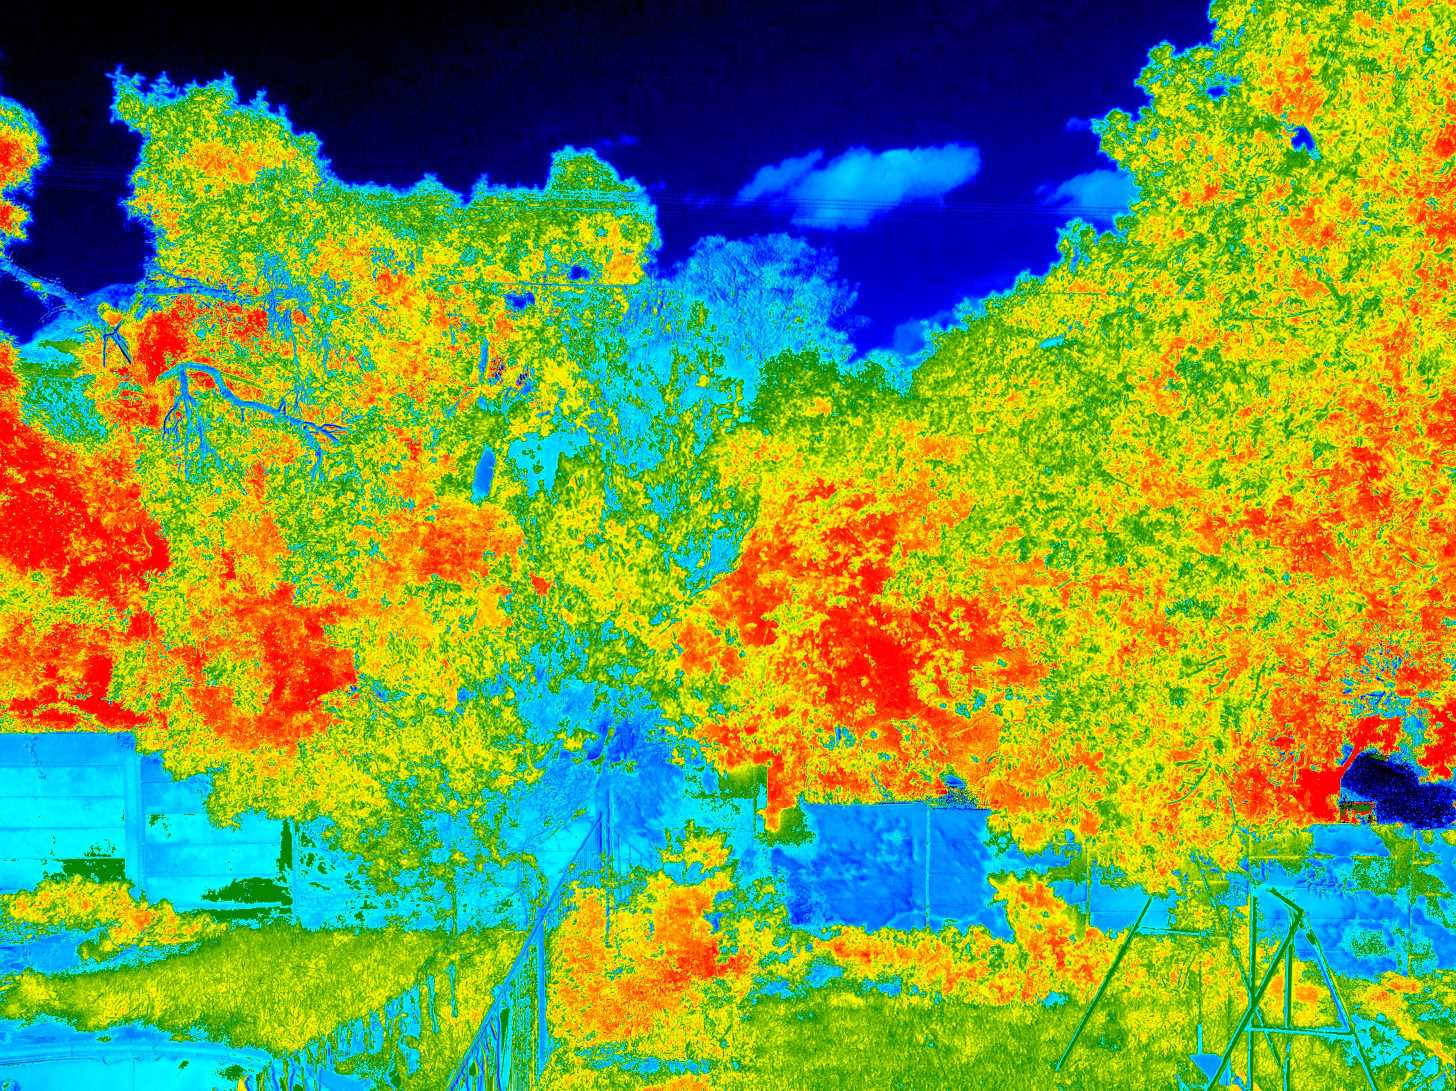
\includegraphics[scale=0.17]{filter/green_d_ndvi.jpg}
\caption{Green filter NDVI (NIR=red, VIS=red)}
\end{subfigure}
\begin{subfigure}{0.5\textwidth}
\centering
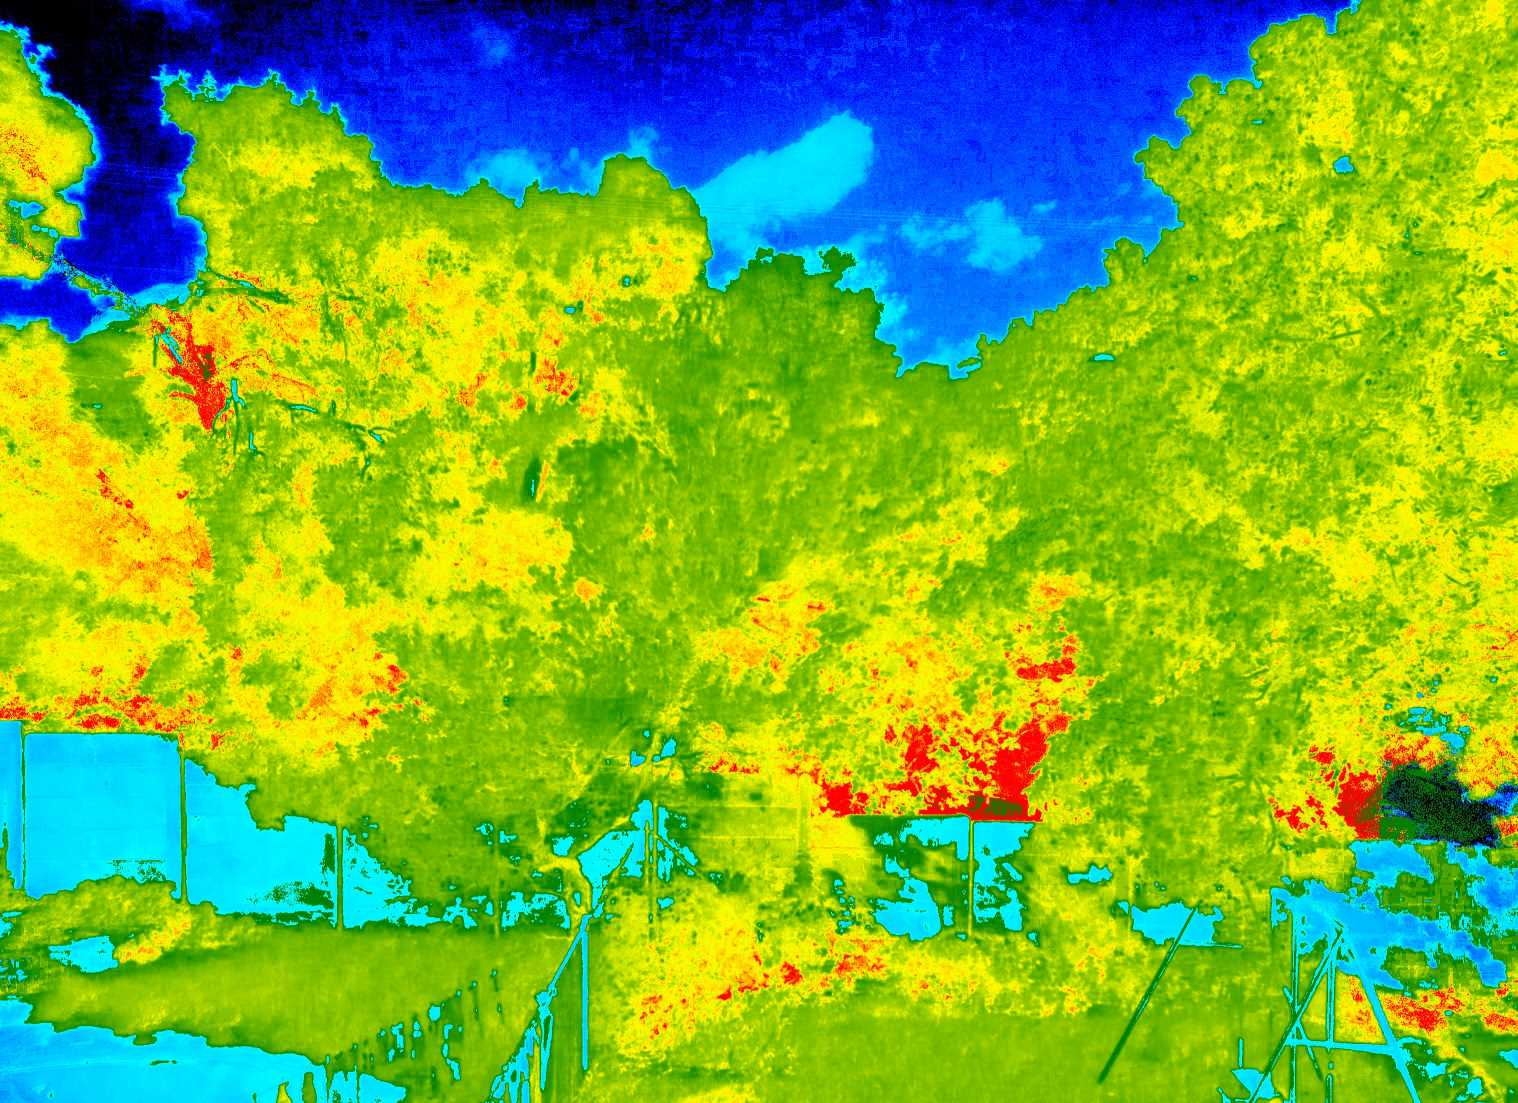
\includegraphics[scale=0.17]{filter/red_Color_Index.jpg}
\caption{Red filter NDVI (NIR=blue, VIS=red)}
\end{subfigure}
\begin{subfigure}{0.5\textwidth}
\centering
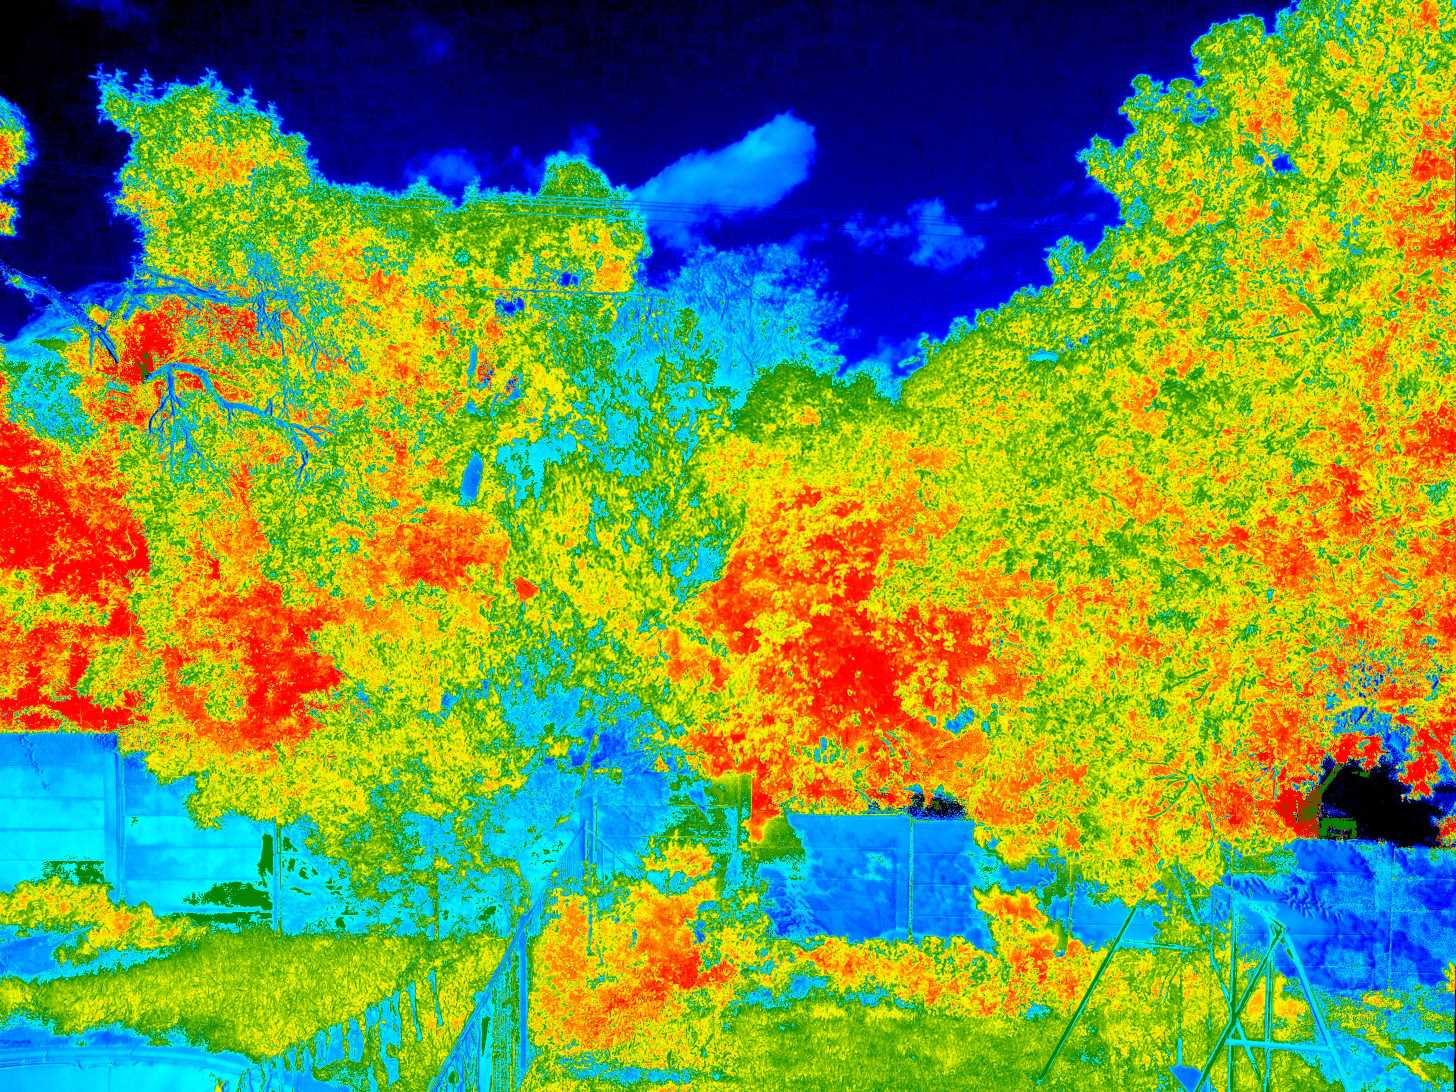
\includegraphics[scale=0.17]{filter/red_d_ndvi.jpg}
\caption{Red filter NDVI (NIR=blue, VIS=red)}
\end{subfigure}
\caption{NDVIs of single (left column) and stereo (right column) filter images}
\label{fig:filters_ndvis}
\end{figure}

\chapter{NDVI Map}
\label{app:ndvi_map}

A large map was produced. The young leaves could be discerned, and had values between 0.5-0.55. This is great news, because the Parrot Sequoia could not discern the leaves having an infra-red camera resolution of only 1.2 MP, as opposed to 8 MP in our application.\\

Cloud processing was used. Final floating-point tiff image is 8842x8283 pixels, at 286 Mb. The processing used 24364 Mb of RAM.\\

\begin{figure}[H]
\begin{subfigure}{0.5\textwidth}
\centering
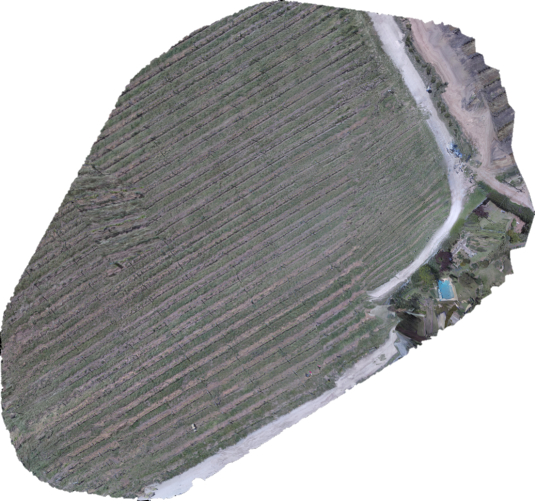
\includegraphics[scale=0.6]{images/map_rgb_large.png}
\caption{RGB map}
\end{subfigure}
\begin{subfigure}{0.5\textwidth}
\centering
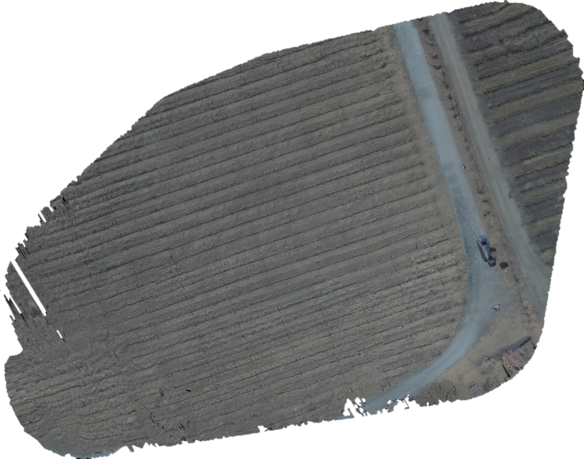
\includegraphics[scale=0.6]{images/map_ir_large.png}
\caption{NIR map}
\end{subfigure}
\caption{Maps processed using MME \cite{mme}}
\label{fig:app_maps}
\end{figure}

\begin{figure}[H]
\centering
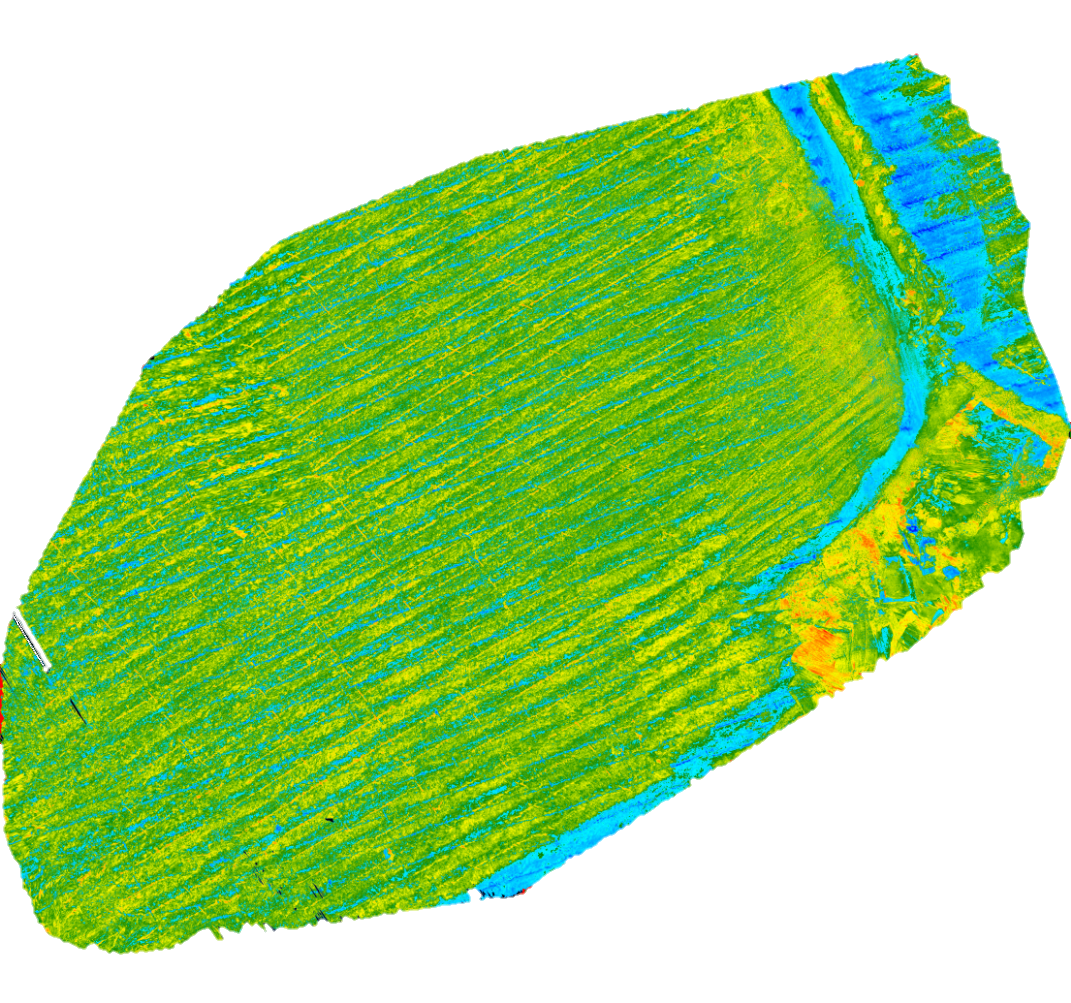
\includegraphics[scale=0.35]{images/map_ndvi_large.png}
\caption{NDVI performed using bUnwarpJ \cite{bunwarpj}}
\label{fig:app_stitch_map}
\end{figure}

\chapter{Chessboard input set}
\label{app:chess}

\begin{figure}[H]
\centering
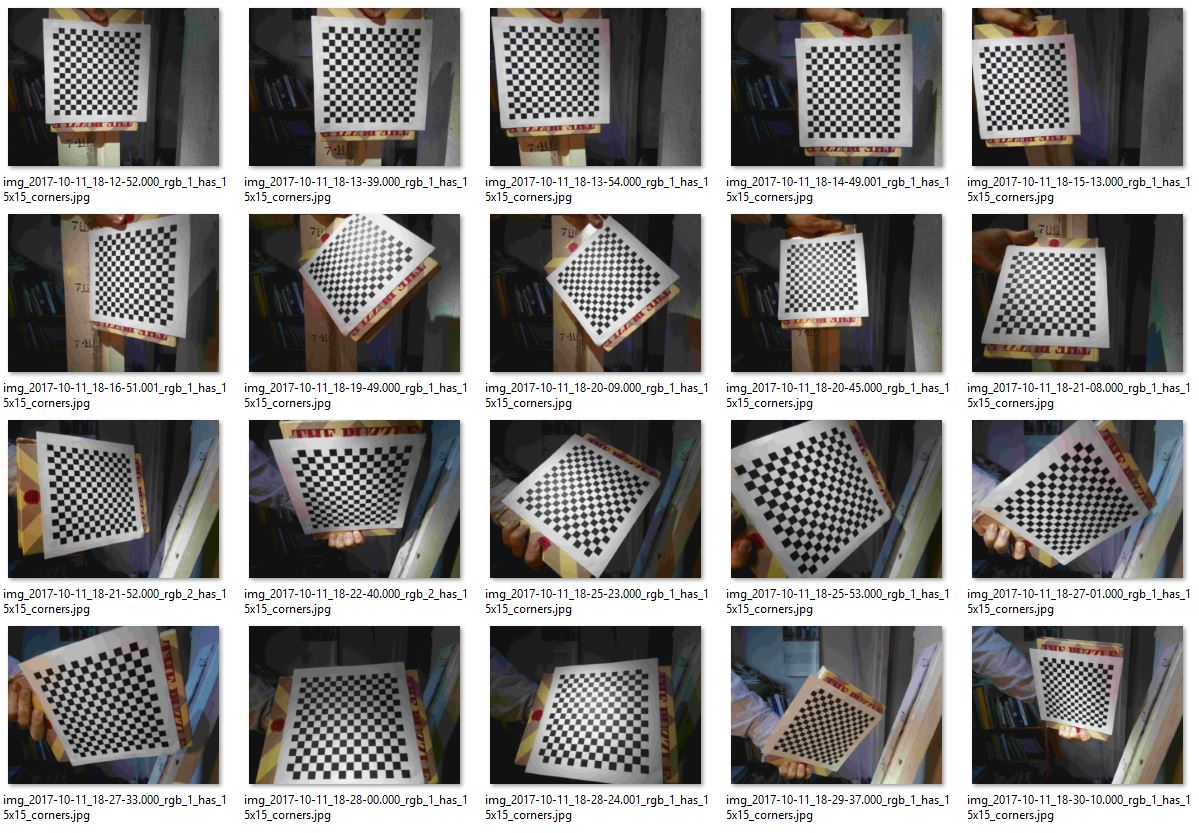
\includegraphics[scale=0.505]{images/rgb_chess_set.JPG}
\caption{RGB input chess images}
\label{fig:rgb_input_chess}
\end{figure}

\begin{figure}[H]
\centering
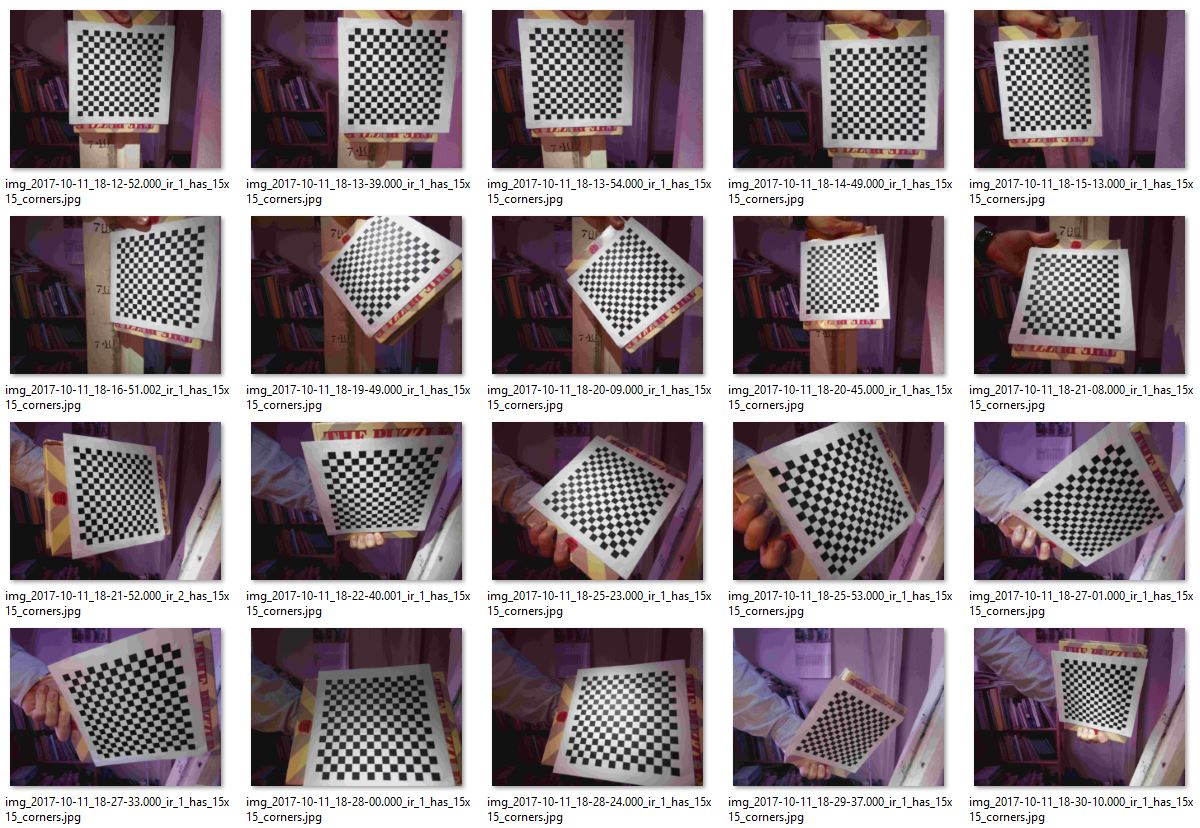
\includegraphics[scale=0.5]{images/ir_chess_set.JPG}
\caption{NIR input chess images}
\label{fig:ir_input_chess}
\end{figure}

\chapter{Stereo calibration and rectification results}
\label{app:stereo_results}

\begin{equation}\label{eq::cm1}
M_c^1 = \begin{bmatrix}
2.523278 & 0 & 1.64 \\
0 & 2.516529 & 1.232 \\
0 & 0 & 0.001
\end{bmatrix}\cdot10^3
\end{equation}

\begin{equation}\label{eq::cm2}
M_c^2 = \begin{bmatrix}
2.505381 & 0 & 1.64 \\
0 & 2.505083 & 1.232 \\
0 & 0 & 0.001
\end{bmatrix}\cdot10^3
\end{equation}

\begin{equation}\label{eq::R}
R = \begin{bmatrix}
999.281 & -6.4992 & 37.35413 \\
6.59547 & 999.97524 & -2.45456 \\
-37.33725 & 2.69917 & 999.29908
\end{bmatrix}\cdot10^3
\end{equation}

\begin{equation}\label{eq::E}
E = \begin{bmatrix}
-0.3150989 & 158.311619 & 35.973848 \\
-55.293721 & -6.403995 & -2757.525727 \\
-18.200605 & 2753.713987 & -8.117986
\end{bmatrix}\cdot10^-3
\end{equation}

\begin{equation}\label{eq::F}
F = \begin{bmatrix}
-2.54558709\cdot10^-6 & 1.28238104\cdot10^-3 & -0.842399343\\
-0.446754\cdot10^-3 & -51.880818\cdot10^-6 & -55.4216639\\
0.1861918 & 53.846 & 1000
\end{bmatrix}\cdot10^-3
\end{equation}

\begin{equation}\label{eq::R1}
R_1 = \begin{bmatrix}
0.99977728 & 0.00654886 & -0.02006268\\
0.00657528 & 0.9999776 & -0.00125126\\
0.02005403 & 0.0013829 & 0.99979794
\end{bmatrix}
\end{equation}

\begin{equation}\label{eq::R2}
R_2 = \begin{bmatrix}
0.99826641 & 0.01319195 & -0.05735987\\
-0.01311635 & 0.99991254 & 0.00169423\\
0.05737721 & -0.00093894 & 0.99835213
\end{bmatrix}
\end{equation}

\begin{equation}\label{eq::P1}
P_1 = \begin{bmatrix}
2505.083324 & 0 & 1778.704819 & 0\\
0 & 2505.083324 & 1231.092529  & 0\\
0 & 0 & 1 & 0
\end{bmatrix}
\end{equation}

\begin{equation}\label{eq::P2}
P_2 = \begin{bmatrix}
2505.083324 &    0.       & 1778.704819 & 6909.840227\\
 0          & 2505.083324 & 1231.092529 &    0        \\
 0          &    0        &    1        &    0         \\
\end{bmatrix}
\end{equation}

\begin{equation}\label{eq::Q}
Q\ =\ \begin{bmatrix}
1 & 0 & 0 & -1.778705\cdot10^3\\
0 & 1 & 0 & -1.231093\cdot10^3\\
0 & 0 & 0 & 2.505083\cdot10^3\\
0 & 0 & -0.362539 & 0
\end{bmatrix}
\end{equation}

\begin{equation}\label{eq::T}
T\ =\ \begin{bmatrix}
2.75354568\\
0.03638771\\
-0.15821732
\end{bmatrix}
\end{equation}

\begin{equation}\label{eq::validpix1}
valid\ Pix\ ROI_1\ =\ 
\begin{bmatrix}
x_1 & y_1\\
x_2 & y_2
\end{bmatrix}\ =
\begin{bmatrix}
88 & 6\\
3192 & 2421
\end{bmatrix}
\end{equation}

\begin{equation}\label{eq::validpix2}
valid\ Pix\ ROI_2\ =\ 
\begin{bmatrix}
x_1 & y_1\\
x_2 & y_2
\end{bmatrix}\ =
\begin{bmatrix}
0 & 26\\
3204 & 2378
\end{bmatrix}
\end{equation}

\begin{equation}\label{eq::error1}
error_1 = 17.255\%
\end{equation}
\begin{equation}\label{eq::error2}
error_2 = 14.647\%
\end{equation}

\chapter{Project Planning}

% Please add the following required packages to your document preamble:
% \usepackage{graphicx}
\begin{table}[H]
\centering
%\caption{My caption}
\label{my-label}
\resizebox{\textwidth}{!}{%
\begin{tabular}{ll}
\textbf{Task Description}             & \textbf{Duration}       \\
Drone construction                    & 7-15 July 2017          \\
First flight attempts                 & 15-17 July 2017         \\
Official commencement of Project E448 & 17 July 2017            \\
Drone calibration, software           & 18 July - 7 August 2017 \\
Camera acquisition                    & 8 August - 3 Sept 2017  \\
Camera calibration                    & 4 Sept - 16 Oct 2017    \\
Flight with Chris on Longridge        & 29 Sept 2017            \\
Image processing                      & 17 - 29 Oct 2017        \\
Report writing                        & 11 Oct 2017             \\
Hand in report                        & 30 Oct 2017            
\end{tabular}%
}
\end{table}


\chapter{Outcome Compliance}

% Please add the following required packages to your document preamble:
% \usepackage{graphicx}
\begin{table}[H]
\centering
%\caption{My caption}
\label{my-label}
\resizebox{\textwidth}{!}{%
\begin{tabular}{ll}
\textbf{Outcome} & \textbf{Criteria} \\
ELO 1. Problem Solving & Chapter 3, 4, 5, 6, Appendices \\
ELO 2. Application of scientific and engineering knowledge & Chapter 2, 3, 4, 5, 6, Appendices \\
ELO 3. Engineering Design & Chapter 3, 4, 5, Appendices \\
ELO 4. Investigations, experiments and data analysis & Chapter 2, 3, 4, 5, 6, Appendices \\
\begin{tabular}[c]{@{}l@{}}ELO 5. Engineering methods, skills and tools, \\ including Information Technology\end{tabular} & Chapter 3, 4, 5, 6, Appendices \\
ELO 6. Professional and technical communication & Chapter 1, 2, 3, 4, 5, 6 \\
ELO 9. Independent Learning Ability & Chapter 2, 3, 4, 5, 6, Appendices
\end{tabular}%
}
\end{table}


\chapter{Code}

Code block \ref{code:getmatrices} shows the method to get camera matrices.

\lstset{language=python,caption={Get matrices},label=code:getmatrices}
\begin{lstlisting}
import cv2 #, numpy, matplotlib
import numpy as np
from matplotlib import pyplot as plt
import glob
import dill
from tqdm import tqdm
import os

##img_type = 'ir'
img_type = 'rgb'
##img_type = 'example'

_x = 15
_y = 15

savefile = img_type + '_matrices_15_dual.pkl'
##root_path = 'C:/Users/d7rob/thesis/chess/master_set/'
root_path = 'C:/Users/d7rob/thesis/chess/15_dual_ethernet/rgb/'
##root_path = 'chess/'
##images = glob.glob('chess/*.jpg')
##images = glob.glob('L:/Backups/thesis/chess/rgb/compressed/picked/*.jpg')
##images = glob.glob('C:/Users/d7rob/thesis/chess/master_set/rgb_7x6/*.jpg')
##images = glob.glob(root_path + img_type + '_7x6/*.jpg')
##images = glob.glob(root_path + img_type + '_15x15/*.jpg')
images = glob.glob(root_path + '/*.jpg')

##gray = 0
# termination criteria
criteria = (cv2.TERM_CRITERIA_EPS + cv2.TERM_CRITERIA_MAX_ITER, 30, 0.001)
# prepare object points, like (0,0,0), (1,0,0), (2,0,0) ....,(6,5,0)
objp = np.zeros((_y*_x,3), np.float32)
objp[:,:2] = np.mgrid[0:_x,0:_y].T.reshape(-1,2)
# Arrays to store object points and image points from all the images.
objpoints = [] # 3d point in real world space
imgpoints = [] # 2d points in image plane.

for fname in tqdm(images):
    print fname
    img = cv2.imread(fname)
    gray = cv2.cvtColor(img, cv2.COLOR_BGR2GRAY)
    # Find the chess board corners
    
    flags = cv2.CALIB_CB_ADAPTIVE_THRESH + \
            cv2.CALIB_CB_NORMALIZE_IMAGE + \
            cv2.CALIB_CB_FILTER_QUADS + \
            cv2.CALIB_CB_FAST_CHECK
##    ret, corners = cv2.findChessboardCorners(gray, (_x,_y), flags)

    ret, corners = cv2.findChessboardCorners(gray, (_x,_y), None, flags)
    # If found, add object points, image points (after refining them)
    if ret == True:
        objpoints.append(objp)
        corners2=cv2.cornerSubPix(gray,corners, (11,11), (-1,-1), criteria)
        imgpoints.append(corners2)
        # Draw and display the corners
        cv2.drawChessboardCorners(img, (_x,_y), corners2, ret)
        draw_path = root_path + os.path.basename(fname)[:-4] + '_'+str(_x)+'x'+str(_y)+'_drawn.jpg'
        print draw_path
        cv2.imwrite(draw_path, img)
##        cv2.imshow('img', img)
##        cv2.waitKey(500)
cv2.destroyAllWindows()

ret, mtx, dist, rvecs, tvecs = cv2.calibrateCamera(objpoints, imgpoints, gray.shape[::-1], None, None)
print ret, mtx, dist, rvecs, tvecs
##img = cv2.imread('C:/Users/d7rob/thesis/chess/rgb/img1_2017-09-25_23-18-52.001_1.jpg')
####img = cv2.imread('chess/left12.jpg')
##h,  w = img.shape[:2]
##newcameramtx, roi=cv2.getOptimalNewCameraMatrix(mtx, dist, (w,h), 1, (w,h))

mean_error = 0
for i in xrange(len(objpoints)):
    imgpoints2, _ = cv2.projectPoints(objpoints[i], rvecs[i], tvecs[i], mtx, dist)
    error = cv2.norm(imgpoints[i], imgpoints2, cv2.NORM_L2)/len(imgpoints2)
    mean_error += error
total_error = mean_error/len(objpoints)
print( "total error: {}".format(total_error) )

dill.dump_session(savefile)

\end{lstlisting}

\newpage
Code block \ref{code:sortcorners} shows the method to sort corner pics from unsuccessful ones.

\lstset{language=python,caption={Sorting potential corner images},label=code:sortcorners}
\begin{lstlisting}
import glob, cv2
import numpy as np
from matplotlib import pyplot as plt

##images = glob.glob('L:/Backups/thesis/chess/rgb/compressed2/picked/*.jpg')
root_dir = 'C:/Users/d7rob/thesis/chess/15_dual_ethernet/compressed'
images = glob.glob(root_dir + '/*.jpg')
print images

for fname in images:
    img = cv2.imread(fname)

    ##gray = cv2.cvtColor(img, cv2.COLOR_RGB2GRAY)
    gray = cv2.cvtColor(img, cv2.COLOR_BGR2GRAY)
    ##gray = img

    ##plt.imshow(gray)
    ##plt.show()

    ##cv2.imshow('gray', gray)
    ##cv2.waitKey(500)
    ##cv2.destroyAllWindows()

    flags = cv2.CALIB_CB_ADAPTIVE_THRESH + \
            cv2.CALIB_CB_NORMALIZE_IMAGE + \
            cv2.CALIB_CB_FILTER_QUADS + \
            cv2.CALIB_CB_FAST_CHECK
##    flags = cv2.CALIB_CB_FAST_CHECK
    ##flags = None
    # 7, 6
##    ret, corners = cv2.findChessboardCorners(gray, (15,15), flags)
    ret, corners = cv2.findChessboardCorners(gray, (15,15), None, flags)

    print np.shape(corners), ret

    if ret == True:
        pass
##        cv2.imwrite((str(fname[:-4]) + '_has_15x15_corners.jpg'), img)

\end{lstlisting}

\newpage
Code block \ref{code:stereorectification} shows the method to stereorectify.

\lstset{language=python,caption={Stereorectification},label=code:stereorectification}
\begin{lstlisting}
import numpy as np
import dill, glob, tqdm

np.set_printoptions(suppress=True)

root_dir = 'C:/Users/d7rob/thesis/distorted'
root_dir = 'L:/Backups/thesis/longridge'

_rgb_name = "/rgb"
_ir_name = "/ir"
rgb_images = glob.glob(root_dir + _rgb_name + '/*.jpg')
ir_images = glob.glob(root_dir + _ir_name + '/*.jpg')
zipped_images = zip(rgb_images, ir_images)

##print ": " + str()
def pp(val):
    print '::\t' + str(val)

class Matrices:
    def __init__(self, total_error, ret, mtx, dist, rvecs, tvecs, imgpoints, objpoints, gray):
        self.total_error = total_error
        self.ret = ret
        self.mtx = mtx
        self.dist = dist
        self.rvecs = rvecs
        self.tvecs = tvecs
        self.imgpoints = imgpoints
        self.objpoints = objpoints
        self.resolution = gray.shape[::-1]

    def print_values(self):
        print 'total_error:\t\t' + str(self.total_error)
        print 'ret:\t\t\t' + str(self.ret)
        print 'mtx.shape:\t\t' + str(self.mtx.shape)
        print 'dist.shape:\t\t' + str(self.dist.shape)
        print 'rvecs.shape:\t\t' + str(np.shape(self.rvecs))
        print 'tvecs.shape:\t\t' + str(np.shape(self.tvecs))
        print 'np.shape(objpoints):\t' + str(np.shape(self.objpoints))
        print 'np.shape(imgpoints):\t' + str(np.shape(self.imgpoints))
        print 'resolution:\t\t' + str(self.resolution)
        print ''
##        print 'imgpoints2.shape:\t' + str(np.shape(imgpoints2))

##savefile = 'rgb_matrices.pkl'
##savefile = 'rgb_matrices_13_print.pkl'
##savefile = 'rgb_matrices_14_dual.pkl'
##savefile = '_matrices_12_ESS.pkl'
savefile = 'rgb_matrices_15_dual.pkl'
dill.load_session(savefile)
rgb = Matrices(total_error, ret, mtx, dist, rvecs, tvecs, imgpoints, objpoints, gray)
rgb.print_values()

##savefile = 'ir_matrices.pkl'
##savefile = 'ir_matrices_13_print.pkl'
##savefile = '_matrices_12_ESS.pkl'
savefile = 'ir_matrices_15_dual.pkl'
dill.load_session(savefile)
ir = Matrices(total_error, ret, mtx, dist, rvecs, tvecs, imgpoints, objpoints, gray)
ir.print_values()

##### find fundamental matrix F
####F, mask = cv2.findFundamentalMat(np.array(rgb.imgpoints[0]), np.array(ir.imgpoints[0]))
####print "F: " + str(F)
####print "mask.shape: " + str(mask.shape)
####print ''
####
##### uncalibrated stereo rectification
####ret, H1, H2 = cv2.stereoRectifyUncalibrated(rgb.imgpoints[0], ir.imgpoints[0], F, rgb.resolution)
####print "stereoRectifyUncalibrated ret: " + str(ret)
####print "H1: " + str(H1)
####print "H2: " + str(H2)
####
####R1 = np.linalg.inv(rgb.mtx)*H1*rgb.mtx
####R2 = np.linalg.inv(ir.mtx)*H2*ir.mtx
####P1 = rgb.mtx
####P2 = ir.mtx
####
####print "R1: " + str(R1)
####print "R2: " + str(R2)
####print "P1: " + str(P1)
####print "P2: " + str(P2)
####print ''

# mono calibration

ret, mtx, dist, rvecs, tvecs = cv2.calibrateCamera(rgb.objpoints, rgb.imgpoints, rgb.resolution, None, None)

# stereo calibration
flags = cv2.CALIB_FIX_ASPECT_RATIO + \
                    cv2.CALIB_ZERO_TANGENT_DIST + \
                    cv2.CALIB_USE_INTRINSIC_GUESS + \
                    cv2.CALIB_SAME_FOCAL_LENGTH + \
                    cv2.CALIB_RATIONAL_MODEL + \
                    cv2.CALIB_FIX_K3 + cv2.CALIB_FIX_K4 + cv2.CALIB_FIX_K5

criteria = (cv2.TERM_CRITERIA_COUNT + cv2.TERM_CRITERIA_EPS, 100, 0.00001)

initCameraMatrix1 = cv2.initCameraMatrix2D(rgb.objpoints, rgb.imgpoints, rgb.resolution, 0);
initCameraMatrix2 = cv2.initCameraMatrix2D(ir.objpoints, ir.imgpoints, ir.resolution, 0);
initDist = np.array([[0]*5])
print "initCameraMatrix1: " + str(initCameraMatrix1)
print "initCameraMatrix2: " + str(initCameraMatrix2)
    
##retval, cameraMatrix1, distCoeffs1, cameraMatrix2, distCoeffs2, R, T, E, F = cv2.stereoCalibrate(rgb.objpoints, rgb.imgpoints, ir.imgpoints, initCameraMatrix1, initDist, initCameraMatrix2, initDist, rgb.resolution, flags, criteria)

retval, cameraMatrix1, distCoeffs1, cameraMatrix2, distCoeffs2, R, T, E, F = cv2.stereoCalibrate(rgb.objpoints, \
                                                                                                 rgb.imgpoints, \
                                                                                                 ir.imgpoints, \
                                                                                                 rgb.resolution,
                                                                                                 initCameraMatrix1, \
                                                                                                 initDist, \
                                                                                                 initCameraMatrix2, \
                                                                                                 initDist, \
                                                                                                 None, None, None, None, \
                                                                                                 criteria, \
                                                                                                 flags)

print "stereoCalibrate retval: " + str(retval)
print "cameraMatrix1: " + str(cameraMatrix1)
print "distCoeffs1: " + str(distCoeffs1)
print "cameraMatrix2: " + str(cameraMatrix2)
print "distCoeffs2: " + str(distCoeffs2)
print "R: " + str(R)
print "T: " + str(T)
print "E: " + str(E)
print "F: " + str(F)
print ''

# stereo rectification
flags = cv2.CALIB_ZERO_DISPARITY
##flags = None

##R1, R2, P1, P2, Q, validPixROI1, validPixROI2 = cv2.stereoRectify(cameraMatrix1, distCoeffs1, cameraMatrix2, distCoeffs2, rgb.resolution, R, T, flags, 1, rgb.resolution)

R1, R2, P1, P2, Q, validPixROI1, validPixROI2 = cv2.stereoRectify(cameraMatrix1, distCoeffs1, cameraMatrix2, distCoeffs2, rgb.resolution, R, T, None, None, None, None, None, flags, 1, rgb.resolution)

print "R1: " + str(R1)
print "R2: " + str(R2)
print "P1: " + str(P1)
print "P2: " + str(P2)
print "Q: " + str(Q)
print "validPixROI1: " + str(validPixROI1)
print "validPixROI2: " + str(validPixROI2)
print ''

# pre-compute undistortion matrices
rgb_mapx, rgb_mapy = cv2.initUndistortRectifyMap(cameraMatrix1, distCoeffs1, R1, P1, rgb.resolution, cv2.CV_32FC1) # 5
ir_mapx, ir_mapy = cv2.initUndistortRectifyMap(cameraMatrix2, distCoeffs2, R2, P2, ir.resolution, cv2.CV_32FC1) # 5

# batch undistortion

for rgb_path, ir_path in tqdm(zipped_images):
    print ''
    rgb_img = cv2.imread(rgb_path)
    dst = cv2.remap(rgb_img, rgb_mapx, rgb_mapy, cv2.INTER_LINEAR)
    rgb_undistort_path = rgb_path[:-4] + '_stereo_undistorted.jpg'
##    print "rgb_undistort_path: " + str(rgb_undistort_path)
##    cv2.rectangle(dst, validPixROI1[:2], validPixROI1[2:],(0, 0, 255),30)
    dst = dst[validPixROI1[1]:validPixROI1[3], validPixROI1[0]:validPixROI1[2]]
    ##$ cv2.imwrite(rgb_undistort_path, dst)

    ir_img = cv2.imread(ir_path)
    dst = cv2.remap(ir_img, ir_mapx, ir_mapy, cv2.INTER_LINEAR)
    ir_undistort_path = ir_path[:-4] + '_stereo_undistorted.jpg'
##    print "ir_undistort_path: " + str(ir_undistort_path)
##    cv2.rectangle(dst, validPixROI2[:2], validPixROI2[2:],(0, 0, 255),30)
    dst = dst[validPixROI2[1]:validPixROI2[3], validPixROI2[0]:validPixROI2[2]]
    ##$ cv2.imwrite(ir_undistort_path, dst)

    # mono output

####    h, w = rgb_img.shape[:2]
####    newcameramtx, roi = cv2.getOptimalNewCameraMatrix(mtx, dist, (w,h), 1, (w,h))
####    print "newcameramtx: " + str(newcameramtx)
####    print "roi: " + str(roi)
####
####    # undistort mono
####    _mapx, _mapy = cv2.initUndistortRectifyMap(mtx, dist, None, newcameramtx, (w,h), cv2.CV_32FC1) # 5
####    _path = rgb_path
####    _img = cv2.imread(_path)
####    _dst = cv2.remap(_img, _mapx, _mapy, cv2.INTER_LINEAR)
####
####    _undistort_path = _path[:-4] + '_mono_undistorted.jpg'
####    cv2.imwrite(_undistort_path, _dst)

\end{lstlisting}

\newpage
Code block \ref{code:duallistmaker} shows the method to create a dual list.

\lstset{language=python,caption={Dual list creator},label=code:duallistmaker}
\begin{lstlisting}
import glob

root_dir = 'C:/Users/d7rob/thesis/distorted/undistorted'
root_dir = 'L:/Backups/thesis/longridge'
root_dir = 'C:/Users/d7rob/thesis/home_lab_window_2'

_rgb_name = "/rgb_blue"
_ir_name = "/ir_blue"
rgb_images = glob.glob(root_dir + _rgb_name + '/*.jpg')
ir_images = glob.glob(root_dir + _ir_name + '/*.jpg')

for x, y in zip(rgb_images, ir_images):
    print y + ', ' + x

\end{lstlisting}


Code block \ref{code:tcp_trigger} shows the method to trigger simultaneously via TCP.

\lstset{language=python,caption={TCP triggering},label=code:tcp_trigger}
\begin{lstlisting}
import socket, os, threading
from threading import Thread
from time import sleep, time

clients = set()
clients_lock = threading.Lock()
camera_mode = False
cameras_triggered = 0
time_now = 0


def listener(_client, _address):
    global camera_mode, cameras_triggered
    print("Accepted connection from: ", _address)
    cameras_triggered += 1
    with clients_lock:
        clients.add(_client)
    try:
        while True:
            data = _client.recv(32)
            print("received: " + repr(data))
            if not data:
                break
            if "CAMERA_MODE_ENABLED" in data:
                camera_mode = True
                for c in clients:
                    c.sendall("ACK")
            if "CAMERA_MODE_DISABLED" in data:
                camera_mode = False
                for c in clients:
                    c.sendall("ACK")
            if "CAMERA_COMPLETE":
                cameras_triggered += 1
    except Exception as e:
        print(e)
    finally:
        with clients_lock:
            clients.remove(_client)
            _client.close()

count = 0


def camera_process():
    global camera_mode, cameras_triggered, clients, time_now, count
    print("Trigger thread ready.")
    while True:
        if camera_mode and cameras_triggered >= len(clients) and len(clients) > 0:
            cameras_triggered = 0
            with clients_lock:
                print("Sending trigger " + repr(count) + " to " + repr(len(clients)) + " clients; last " + repr(time() - time_now) + ".")
                count += 1
                time_now = time()
                for c in clients:
                    c.sendall("TRIGGER_NOW")
        sleep(0.001)

t = Thread(target=camera_process)
t.daemon = True
t.start()

#host = 'localhost'
host = ''
port = 10017

s = socket.socket()
s.setsockopt(socket.SOL_SOCKET, socket.SO_REUSEADDR, 1)
s.bind((host, port))
s.listen(3)
th = []

try:
    while True:
        print("Server is listening for connections...")
        client, address = s.accept()
        print ("hi")
        t = Thread(target=listener, args=(client, address))
        t.daemon = True
        th.append(t.start())
except KeyboardInterrupt as e:
    print(e)
\end{lstlisting}

Code block \ref{code:init_mav} shows the method to initialize mavlink.

\lstset{language=bash,caption={Initialize mavlink},label=code:init_mav}
\begin{lstlisting}
#!/bin/bash

echo "MAVlink initialisation started."

arg1=
start=true
PREV_IP_GCS=
while true ; do
	sleep 0.5
	IP_GCS="`ping -I wlan0 -c1 rod693a | sed -nE 's/^PING[^(]+\(([^)]+)\).*/\1/p'`"
	if ((${#IP_GCS})); then
		printf "Ground Control Station IP address is %s\n" "$IP_GCS"
		#arg1="--out $IP_GCS:14550"
		arg1="-e $IP_GCS:14550"
		if ! [ "$IP_GCS" = "$PREV_IP_GCS" ] ; then start=true ; fi
		PREV_IP_GCS=$IP_GCS
	else
		unset arg1
	fi
	if [ "$start" = true ] ; then
		#sudo pkill -f "mavproxy.py"
		sudo pkill -f "mavlink-routerd"
		#cmd="mavproxy.py --daemon --master localhost:14550 --out localhost:14850 --out 169.254.169.254:14850 $arg1"
		cmd="/home/pi/mavlink-router/mavlink-routerd 0.0.0.0:14550 -e localhost:14850 -e 169.254.169.254:14850 $arg1"
		echo $cmd
		$cmd &
		start=false
	fi
	sleep 4.5
done

\end{lstlisting}

Code block \ref{code:wifiup} shows the method to reconnect wifi.

\lstset{language=bash,caption={Wifi reconnnection},label=code:wifiup}
\begin{lstlisting}
#!/bin/bash

echo "Wifi reconnection monitor started."

while true ; do
  if iwconfig wlan0 | grep -q "ESSID:off" ; then
    echo "Network connection down! Attempting reconnection."
    ifup --force wlan0
  fi
  sleep 5
done

\end{lstlisting}

Code block \ref{code:rc_local} shows the method to boot scripts.

\lstset{language=bash,caption={Scripts on-boot},label=code:rc_local}
\begin{lstlisting}
#!/bin/sh -e
#
# rc.local
#
# This script is executed at the end of each multiuser runlevel.
# Make sure that the script will "exit 0" on success or any other
# value on error.
#
# In order to enable or disable this script just change the execution
# bits.
#
# By default this script does nothing.

# Print the IP address
_IP=$(hostname -I) || true
if [ "$_IP" ]; then
  printf "My IP address is %s\n" "$_IP"
fi

su - pi -c "screen -dmS wifi sudo /home/pi/re_wlan.sh"
su - pi -c "screen -dmS mav ~/init_mav.sh"
su - pi -c "screen -dmS cam python ~/thesis-image-processing/dronekit/capture_mode.py"

exit 0

\end{lstlisting}

Code block \ref{code:interfaces} shows the method interfaces file.

\lstset{language=bash,caption={Interfaces file},label=code:interfaces}
\begin{lstlisting}
# interfaces(5) file used by ifup(8) and ifdown(8)

# Please note that this file is written to be used with dhcpcd
# For static IP, consult /etc/dhcpcd.conf and 'man dhcpcd.conf'

# Include files from /etc/network/interfaces.d:
source-directory /etc/network/interfaces.d

auto lo
iface lo inet loopback

allow-hotplug intwifi0
iface intwifi0 inet manual
    wpa-conf /etc/wpa_supplicant/wpa_supplicant.conf

allow-hotplug wlan0
iface wlan0 inet manual
    wpa-conf /etc/wpa_supplicant/wpa_supplicant.conf

allow-hotplug wlan1
iface wlan1 inet manual
    wpa-roam /etc/wpa_supplicant/wpa_supplicant.conf

allow-hotplug eth0
iface eth0 inet manual

iface default inet dhcp

\end{lstlisting}

Code block \ref{code:arducopter} shows the method to connect arducopter.

\lstset{language=bash,caption={Arducopter connections file},label=code:arducopter}
\begin{lstlisting}
# Default settings for ArduPilot for Linux.
# The file is sourced by systemd from arducopter.service

#TELEM1="-A tcp:127.0.0.1:5763:wait"
TELEM1="-A udp:127.0.0.1:14550"
TELEM2="-C /dev/ttyAMA0"
TELEM3="-D udp:10.0.0.95:14550"
#TELEM3="-D udp:0.0.0.0:14250"
TELEM4="-C /dev/ttyUSB0"
TELEM5="-C /dev/ttyUSB1"

# Options to pass to ArduPilot
ARDUPILOT_OPTS="$TELEM1 $TELEM2 $TELEM3" #$TELEM4 $TELEM5"

                          #    # ###### #      #####
                          #    # #      #      #    #
                          ###### #####  #      #    #
                          #    # #      #      #####
                          #    # #      #      #
                          #    # ###### ###### #

# -A is a console switch (usually this is a Wi-Fi link)

# -C is a telemetry switch
# Usually this is either /dev/ttyAMA0 - UART connector on your Navio
# or /dev/ttyUSB0 if you're using a serial to USB convertor

# -B or -E is used to specify non default GPS

# Type "emlidtool ardupilot" for further help
\end{lstlisting}

Code block \ref{code:simultaneous} shows the method to trigger simultaneous shots.

\lstset{language=python,caption={Potential packet},label=code:simultaneous}
\begin{lstlisting}
from dronekit import connect, VehicleMode
from threading import Thread
from time import sleep, time
# import datetime as dt
from datetime import datetime, timedelta
import socket, os, threading, sys
import picamera

UDP_IP = "169.254.169.254"
UDP_PORT = 5005

# Connect to UDP endpoint.
connecting_bool = True
while connecting_bool:
  try:
    print "Connecting to UDP endpoint."
    vehicle = connect('0.0.0.0:14850', wait_ready=True)
    if vehicle: connecting_bool = False
  except KeyboardInterrupt:
    connecting_bool = False
    sys.exit(0)
  except Exception as e:
    print e

camera = picamera.PiCamera()
camera.resolution = (3280, 2464)
camera.start_preview()

print " Mode: %s" % vehicle.mode.name
print vehicle.channels['1']

##print "Autopilot Firmware version: %s" % vehicle.version
##print "Autopilot capabilities (supports ftp): %s" % vehicle.capabilities.ftp
##print "Global Location: %s" % vehicle.location.global_frame
##print "Global Location (relative altitude): %s" % vehicle.location.global_relative_frame
##print "Local Location: %s" % vehicle.location.local_frame    #NED
##print "Attitude: %s" % vehicle.attitude
##print "Velocity: %s" % vehicle.velocity
##print "GPS: %s" % vehicle.gps_0
##print "Groundspeed: %s" % vehicle.groundspeed
##print "Airspeed: %s" % vehicle.airspeed
##print "Gimbal status: %s" % vehicle.gimbal
##print "Battery: %s" % vehicle.battery
##print "EKF OK?: %s" % vehicle.ekf_ok
##print "Last Heartbeat: %s" % vehicle.last_heartbeat
##print "Rangefinder: %s" % vehicle.rangefinder
##print "Rangefinder distance: %s" % vehicle.rangefinder.distance
##print "Rangefinder voltage: %s" % vehicle.rangefinder.voltage
##print "Heading: %s" % vehicle.heading
##print "Is Armable?: %s" % vehicle.is_armable
##print "System status: %s" % vehicle.system_status.state
##print "Mode: %s" % vehicle.mode.name    # settable
##print "Armed: %s" % vehicle.armed    # settable

#@vehicle.on_attribute('location')
#def listener(self, attr_name, value):
    # `self`: :py:class:`Vehicle` object that has been updated.
    # `attr_name`: name of the observed attribute - 'location'
    # `value` is the updated attribute value (a :py:class:`Locations`). This can be queried for the frame information
    #print " Global: %s" % value.global_frame
    #print " GlobalRelative: %s" % value.global_relative_frame
    #print " Local: %s" % value.local_frame

@vehicle.on_message('MAV_CMD_DO_DIGICAM_CONTROL')
def my_method(self, name, msg):
    print " name: %s" % name
    print " msg: %s" % msg

@vehicle.on_message('CAMERA_TRIGGER')
def my_method2(self, name, msg):
    print " name: %s" % name
    print " msg: %s" % msg

last_trigger_time = 0
cam_count = 0
trigger_count = 0
@vehicle.on_message('CAMERA_FEEDBACK')
def process_camera(self, name, msg):
    global last_trigger_time, camera, trigger_count
    trigger_count += 1
    if (trigger_count % 2):
        pass
      #print msg.time_usec
      ##take_photo(msg.time_usec)
    #if time() - last_trigger > 1.0/2:
        #print " name: %s" % name
        #print " msg: %s" % msg
        #print msg.time_usec
    #   last_trigger = time()
    #   missed=0
    #    cam_count += 1
    #else:
    #   if (missed % 2 > 0):
    #       print "missed_" + datetime.datetime.now().strftime('%Y-%m-%d_%H-%M-%S.%f')[:-3]
    #   missed += 1
    
def wait():
    # Calculate the delay to the start of the next hour
    next_sec = (datetime.now() + timedelta(seconds=1)).replace(microsecond=0)
    delay = (next_sec - datetime.now()).microseconds/1000000.0
    # print "delay: " + repr(delay)
    sleep(delay)

def take_photo():
    global cam_count
    cam_count += 1
    dir = '/home/pi/images/'
    os.system("mkdir -p " + dir)
    wait()
    string = dir + 'img_' + datetime.now().strftime('%Y-%m-%d_%H-%M-%S.%f')[:-3] + '_rgb_' + str(cam_count) + '.jpg'
    print string
    #string2 = dir + 'img2_' + time.strftime("%Y-%m-%d_%H-%M-%S_", time.gmtime(t/1000000)) + str(t)[-6:-3] + '_' + str(cam_count) + '.jpg'
    # print string2
    # sleep(0.5)
    camera.capture(string)
    # time.sleep(0.2)

"""
sock = socket.socket()
ack = False
connected = False


def process_data():
    global sock, ack, connected
    while not connected:
        try:
            sock = socket.socket()
            if not sock.connect(('localhost', 10017)):
              connected = True
        except Exception as e:
          print(e)
    try:
        while True:
            data = sock.recv(32)
            # print("data: " + repr(data))
            if "KEEP_ALIVE" in data:
                sock.sendall("KEEP_ALIVE")
            if "ACK" in data:
                ack = True
            if "TRIGGER_NOW" in data and camera_mode:
                take_photo(0)
                sock.sendall("CAMERA_COMPLETE1")
    except Exception as e:
        print(e)
    finally:
        sock.close()
"""

#Create a message listener for all messages.
#@vehicle.on_message('*')
#def listener(self, name, message):
#    print name
#    if 'CAMERA_FEEDBACK' in name:
# print message
#    print 'message: %s' % message

"""
t = Thread(target=process_data)
t.daemon = True
t.start()
"""

camera_mode = False
prev_cam_mode = False
# cam_count = 0

try:
  while True:
      camera_mode = vehicle.channels['8'] > 1100# or True
      if camera_mode:
        take_photo()
      else:
        cam_count = 0
      # if camera_mode != prev_cam_mode:
      #   ack = False
      # if camera_mode:
      #   if not ack and connected:
      #     sock.sendall("CAMERA_MODE_ENABLED1")
      # else:
      #   if not ack and connected:
      #     sock.sendall("CAMERA_MODE_DISABLED1")
      # prev_cam_mode = camera_mode
      sleep(0.01)
except Exception as e:
  print e

\end{lstlisting}

Code block \ref{code:pi_setup} shows the methods to setup Raspberry Pi.

\lstset{language=bash,caption={Raspberry Pi setup},label=code:pi_setup}
\begin{lstlisting}
###############################################################
Enable hostname on windows
###############################################################

$ sudo apt-get update

On the Raspberry Pi you need to install samba and winbind
$ sudo apt-get install samba
$ sudo apt-get install winbind

# to read windows hostname
$ sudo apt-get install libnss-winbind

Edit /etc/nsswitch.conf to enable wins
change 'hosts: files dns' TO 'hosts: files wins dns'

To change the hostname
edit /etc/hostname

FYI 'raspberrypi' works just fine as a host name

$ sudo reboot

###############################################################
Setup arducopter for quad
###############################################################

$ sudo update-alternatives --config arducopter
15

$ sudo nano /etc/default/arducopter 
127.0.0.1 -> 10.0.0.95

$ sudo systemctl daemon-reload

sudo systemctl start arducopter

sudo systemctl enable arducopter

###############################################################
Setup Samba for network drive share
###############################################################

sudo smbpasswd -a pi
sudo smbpasswd -a root
sudo nano /etc/samba/smb.conf

[root_fs]
path = /
valid users = root
read only = no

[pi_fs]
path = /home/pi
valid users = pi
read only = no

sudo service smbd restart

# in windows, win key + R, \\navio


###############################################################
Dronekit setup
###############################################################

sudo pip install dronekit
sudo pip install dronekit-sitl


###############################################################
MAVProxy
###############################################################
sudo apt-get install python-dev python-opencv python-wxgtk3.0 python-pip python-matplotlib python-pygame python-lxml
pip install MAVProxy

# in /etc/rc.local
echo "Starting MAVproxy."
mavproxy.py --out ROD693A:14550 --master localhost:14550 --out localhost:14850 &

###############################################################
PiCamera
###############################################################
sudo apt-get install python-picamera

###############################################################
ssh-key
###############################################################
ssh-keygen -t rsa -C pi@navio
ssh-keygen -t rsa -C pi@infrapi

###############################################################
twisted.internet
###############################################################
pip install twisted


###############################################################
mavlink-router
###############################################################
sudo apt-get install dh-autoreconf
https://github.com/01org/mavlink-router



http://raspberrypi.tomasgreno.cz/ntp-client-and-server.html

sudo apt-get install screen


git remote set-url origin --push --add https://daniel_leonard_robinson@github.com/daniel-leonard-robinson/thesis-image-processing.git
\end{lstlisting}

\end{appendices}